% Core.Tex, version=13
% Satin Dmitri, 2016-2018

% Changelog:
% 13: Add No Title mode
% 12.1: Improve \N, \Q, \R, \Z, \CC definitions a bit, add some customizations for moth mode
% 12: Improve \TODO, \skip[sub][sub]section (takes optional counter now), fix code a bit, add exec end.
% 11: Add cmap
% 10.6: Styling changes
% 10.5: Add \slashn stuff, custom theorem namespace support, style changes.
% 10.4: replace \emptyset in math mode.
% 10.3: add properties(theorems), add \ref example, add \ThmSpacing configure var.
% 10.2: fix for proofs
% 10.1: better style for theorems, thmslashn
% 10: more math symbols, theorems support (\enablemath), using paralist, using cancel, moved code support to \enablecode
% 9: new math symbols (\enablemath), \skip[sub][sub]section, \CustomTitle support
% 8: better source code support, padding.
% 7: custom head, foot, sections.

\documentclass[a4paper,12pt]{article}
%\usepackage{cmap}
\usepackage[usenames,dvipsnames]{xcolor}
%\usepackage{polyglossia}
\usepackage{xspace}
%\setdefaultlanguage[spelling=modern]{russian}
%\setotherlanguage{english}
%\defaultfontfeatures{Ligatures={TeX},Renderer=Basic}
%\setmainfont[Ligatures={TeX,Historic}]{CMU Serif}
%\setsansfont{CMU Sans Serif}
%\setmonofont{CMU Typewriter Text}
\let\CYRDZE\relax
\usepackage{graphicx}
\graphicspath{ {./images/} }

\pagestyle{plain}
\usepackage[
  left=0.50in,
  right=0.50in,
  top=0.8in,
  bottom=0.7in,
  headheight=0.8in]{geometry}
\pagenumbering{gobble}

\setlength{\parskip}{0.15cm}

\usepackage{indentfirst}

\usepackage{hyperref}
\hypersetup{
  colorlinks,
  citecolor=black,
  filecolor=black,
  linkcolor=blue,
  urlcolor=blue
}

\usepackage{paralist}
\usepackage{cancel}
\usepackage{textcomp}
\usepackage{gensymb}
\usepackage{mdframed}
\usepackage{lastpage}
\usepackage{microtype}
\usepackage[super]{cite}
\usepackage{fancyhdr}
\pagestyle{fancy}

% Основано на коде С. Копелиовича.
\newcommand\Section[2]{
  \newpage % new page
  \stepcounter{section}
  \bigskip
  \phantomsection
  \addcontentsline{toc}{section}{\arabic{section}. #1}
  \begin{center}
    {\huge \bf \arabic{section}. #1}\\
  \end{center}
  \bigskip
  \gdef\SectionName{#1}
  \gdef\AuthorName{#2}

  \lhead{\ShortCourseName}
  \chead{}
  \rhead{\SectionName}

  \cfoot{
%    \topskip0pt\vspace*{\fill}
    \thepage~of~\pageref*{LastPage}
%    \vspace*{\fill}
  }
  
  \renewcommand{\headrulewidth}{0.15 mm}

  \ifx\LaconicFooter\undefined
  \lfoot{
%    \topskip0pt\vspace*{\fill}
    Chapter \texttt{\#\arabic{section}}
%    \vspace*{\fill}
  }
  \rfoot{
%    \topskip0pt\vspace*{\fill}
    Author: \AuthorName
%    \vspace*{\fill}
  }
  \renewcommand{\footrulewidth}{0.15 mm}
  \fi
}

\newcommand\Subsection[1]{
  % Пока здесь нет никаких кастомизаций,
  % Но рекомендуется использовать имено вариацию с большой буквы,
  % На случай, если в будущем они появятся.
  \subsection{#1}
}

\newcommand\Subsubsection[1]{
  % Пока здесь нет никаких кастомизаций,
  % Но рекомендуется использовать имено вариацию с большой буквы,
  % На случай, если в будущем они появятся.
  \subsubsection{#1}
}

\newcommand\slashnl{~\\*[-26pt]}
\newcommand\slashn{~\\*[-22pt]}
\newcommand\slashns{~\\*[-18pt]}
\newcommand\slashnss{~\\*[-14pt]}
\newcommand\slashnsss{~\\*[-10pt]}

\newcommand{\makegood}{
  \ifx\ShortCourseName\undefined
  \gdef\ShortCourseName{\CourseName}
  \fi
  
  % \new command\Custom Title{...} до \make good для того, чтобы
  % переопределить содержимое титульной страницы до содержания.

  \ifx\NoTitlePage\undefined
  
  \ifx\CustomTitle\undefined
    \title{\CourseName}
    \maketitle
  \else
    \pagestyle{empty}
    \CustomTitle
  \fi
  \tableofcontents
  \pagebreak
  \fi
  
  \pagestyle{fancy}
  \pagenumbering{arabic}
  \setcounter{page}{1}

  \lhead{\ShortCourseName}
  
  \ifdefined\ENABLEDMATH
  \renewcommand\proofname{\em\textbf{Proof}}
  \else
  \fi
}

% Использовать как \skipsection или \skipsection[2]

\newcommand\skipsection[1][1]{
  \addtocounter{section}{#1}
}

\newcommand\skipsubsection[1][1]{
  \addtocounter{subsection}{#1}
}

\newcommand\skipsubsubsection[1][1]{
  \addtocounter{subsubsection}{#1}
}

\newcommand{\TODO}[1][]{
  \vspace{0.2em}
  \textbf{{\bf\color{red} TODO:} #1}
  \vspace{0.2em}
}

% Должна использоваться вне \document.
\newcommand\enablemath{
  \usepackage{amsmath,amsthm,amssymb,mathtext}
  \usepackage{thmtools}
  \usepackage{tikz}

  \newcommand\R{\ensuremath{\mathbb{R}}\xspace}
  \newcommand\Q{\ensuremath{\mathbb{Q}}\xspace}
  \newcommand\N{\ensuremath{\mathbb{N}}\xspace}
  \newcommand\Z{\ensuremath{\mathbb{Z}}\xspace}
  \newcommand\CC{\ensuremath{\mathbb{C}}\xspace} % C.C. from Code Geass

  \DeclareRobustCommand{\divby}{%
    \mathrel{\vbox{\baselineskip.65ex\lineskiplimit0pt\hbox{.}\hbox{.}\hbox{.}}}%
  }
  \newcommand\notmid{\centernot\mid}
  
  \let\Im\relax % Переопределяем стрёмные значки для понятных вещей.
  \let\Re\relax
  \DeclareMathOperator\Im{Im}
  \DeclareMathOperator\Re{Re}
  
  \DeclareMathOperator*{\lcm}{lcm}
  \newcommand\vphi{\varphi}
  
  \usepackage{
    nameref,
    hyperref,
    cleveref}

  \ifx\ThmSpacing\undefined
  \def\ThmSpacing{9pt}
  \fi

  \ifx\ThmNamespace\undefined
  \def\ThmNamespace{subsection}
  \fi
  
  \declaretheoremstyle[
    spaceabove=\ThmSpacing, spacebelow=\ThmSpacing,
    headfont=\slshape\bfseries,
    bodyfont=\normalfont,
    postheadspace=0.5em,
  ]{thmstyle_def}

  \declaretheoremstyle[
    spaceabove=\ThmSpacing, spacebelow=\ThmSpacing,
    postheadspace=0.5em,
  ]{thmstyle_thm}

  \declaretheoremstyle[
    spaceabove=\ThmSpacing, spacebelow=\ThmSpacing,
    headfont=\itshape\bfseries,
    notefont=\itshape\bfseries, notebraces={}{},
    bodyfont=\normalfont,
    postheadspace=0.5em,
  ]{thmstyle_cons}

  \declaretheoremstyle[
    spaceabove=\ThmSpacing, spacebelow=\ThmSpacing,
    headfont=\bfseries,
    notefont=\bfseries, notebraces={}{},
    bodyfont=\normalfont,
    postheadspace=0.5em,
  ]{thmstyle_examp}  

  \declaretheoremstyle[
    spaceabove=\ThmSpacing, spacebelow=\ThmSpacing,
    headfont=\ttfamily\itshape,
    notefont=\ttfamily\itshape, notebraces={}{},
    bodyfont=\normalfont,
    postheadspace=0.5em,
  ]{thmstyle_remark}
  
  \declaretheorem[numberwithin=\ThmNamespace, name=Theorem, style=thmstyle_thm]{theorem}
  \declaretheorem[numberwithin=\ThmNamespace, name=Definition, style=thmstyle_def]{definition}
  \declaretheorem[numberwithin=\ThmNamespace, name=Statement, style=thmstyle_thm]{statement}
  \declaretheorem[numberwithin=\ThmNamespace, name=Proposition, style=thmstyle_thm]{proposition}
  \declaretheorem[numberwithin=\ThmNamespace, name=Corollary, style=thmstyle_thm]{corollary}
  \renewcommand{\thetheorem}{\arabic{theorem}}
  \renewcommand{\thedefinition}{\arabic{definition}}
  \renewcommand{\thestatement}{\arabic{statement}}
  \renewcommand{\theproposition}{\arabic{proposition}}
  \renewcommand{\thecorollary}{\arabic{corollary}}
  \declaretheorem[numbered=no, name=Remark, style=thmstyle_remark]{remark}
  \declaretheorem[numbered=no, name=Lemma, style=thmstyle_thm]{lemma}
  \declaretheorem[numbered=no, name=Consequence, style=thmstyle_cons]{consequence}
  \declaretheorem[numbered=no, name=Example, style=thmstyle_examp]{example}
  \declaretheorem[numbered=no, name=Properties, style=thmstyle_cons]{properties}
  \declaretheorem[numbered=no, name=Property, style=thmstyle_cons]{property}
  \declaretheorem[numbered=no, name=Exercise, style=thmstyle_examp]{exerc}
  
  % написать после \begin{proof} и т.п., чтобы
  % продолжить на новой строчке.
  % Вообще рекомендуется использовать \slashn[...].
  \newcommand\thmslashn{\slashn}
  
  % Примеры:
  % Первый, простейший:
  % \begin{theorem} theorem-statement \end{theorem}
  %
  % Второй, использовать название теоремы в заголовке.
  % \begin{definition}[My name] the definition \end{definition}
  %
  % Третий, создать метку, чтобы потом можно было сделать сюда ссылку.
  % \begin{statement}\label{stm:identifier} the statement \end{statement}
  %
  % Четвёртый: ссылки (чтобы понять, в чём разница, нужно собрать и посмотреть).
  % \begin{statement}\label{otherlabel}
  %   Согласно \hyperref[stm:identifier]{Теореме о волшебных палочках} магия существует.
  %   \ref{stm:identifier}
  %   \autoref{stm:identifier} ‘‘\nameref{stm:identifier}’’,
  % \end{statement}
    
  \newcommand\eps{\varepsilon}
  \renewcommand\le{\leqslant}
  \renewcommand\ge{\geqslant}
  \newcommand\empysetold{\emptyset}
  \renewcommand\emptyset{\varnothing}
  
  \newcommand\ENABLEDMATH{YES}
}

\newcommand\enablecode{
  \usepackage{listings}
  \lstset{
    belowcaptionskip=1\baselineskip,
    breaklines=true,
    frame=L,
    xleftmargin=\parindent,
    showstringspaces=false,
    basicstyle=\footnotesize\ttfamily,
    keywordstyle=\bfseries\color{blue},
    commentstyle=\itshape\color{Maroon},
    identifierstyle=\color{black},
    stringstyle=\color{orange},
    numbers=left
  }

  % Some voodoo magic:
  % При желании можно адаптировать цвета под себя,
  % Для этого скопируйте это в conspect.tex с новым названием стиля и отредактируйте
  % Соответствующие куски.
  \lstdefinestyle{supercpp} {
    language=C++,
    deletekeywords={int, long, char, short, unsigned, signed,
      uint64\_t, int64\_t, uint32\_t, int32\_t, uint16\_t, int16\_t, uint8\_t, int8\_t,
      size\_t, ptrdiff\_t, \#include,\#define,\#if,\#ifdef,\#ifndef},
    classoffset=1,
    morekeywords={vector,stack,queue,set,map,unordered\_set,unordered\_map,deque,array,string,multiset,multimap,
      int, long, char, short, unsigned, signed,
      uint64\_t, int64\_t, uint32\_t, int32\_t, uint16\_t, int16\_t, uint8\_t, int8\_t,
      size\_t, ptrdiff\_t
    },
    keywordstyle=\bfseries\color{green!40!black},
    classoffset=0,
    classoffset=2,
    morekeywords={std},
    keywordstyle=\bfseries\color{ForestGreen},
    classoffset=0,
    more comment=[l][\bfseries\color{purple!99!black}]{\#}
  }
}

\usepackage{tabularx}
\usepackage{systeme}
\usepackage{centernot}
\usepackage{mathtools}
%\usepackage{ulem}
\usepackage{enumitem}
\usepackage{amsmath}
\usepackage{float}
\usepackage{hyperref}
\usepackage{pgfplots}
\usepgfplotslibrary{external}
\tikzexternalize
\usepgfplotslibrary{fillbetween}
\pgfplotsset{compat=1.18}
\usetikzlibrary{fpu}
\usetikzlibrary{arrows.meta}

\enablemath

\DeclarePairedDelimiter\abs{\lvert}{\rvert}%
\DeclarePairedDelimiter\norm{\lVert}{\rVert}%
\makeatletter
\let\oldabs\abs
\def\abs{\@ifstar{\oldabs}{\oldabs*}}

\begin{document}
\gdef\CourseName{Numerical Methods}
\author{Notes by Lev Leontev\\Professor: Stephan Juricke}
\makegood
%\subsection{Idk}

\begin{definition}[Numerical Methods]
    Numerical Methods are algorithmic approaches to numerically solve mathematical problems.
    We use them often when it is hard/difficult/impossible to solve a problem analytically.
\end{definition}

\section{Taylor series}
Given a function $f : \mathbb{R} \to \mathbb{R}$
(that is hard to evaluate for some $x \in \mathbb{R}$),
but $f$ and $f^{(n)}$ are known for a value $c$, which is close to $x$.
Can we use this information to approximate $f(x)$?

We know values for $\cos^{(n)}(0)$.
\[
    \begin{cases}
        f(0) = \cos(0) = 1\\
        f'(0) = -\sin(0) = 0\\
        f''(0) = -\cos(0) = -1\\
    \end{cases} \text{ for } c = 0
\]
Can we get $\cos(0.1)$ from this?

\begin{definition}[Taylor series]
    Let $f : \mathbb{R} \to \mathbb{R}$, differentiable 
    infinitely many times at $c \in \mathbb{R}$.
    So we have $f^{(k)}(c),\ k=1,2,\dots $. Then the Taylor series of $f$ at $c$ is:
    \[
        f(x) \approx f(c) + \frac{f(c)}{1!}(x-c)^1 + \frac{f''(c)}{2!}(x-c)^2 + \dots =
        \sum_{k=0}^{\infty} \frac{f^{(k)}}{k!} (x - c)^k
    \]
\end{definition}

\begin{remark}
    Taylor series is a power series.
\end{remark}

\begin{remark}
    For $c = 0$ also known as Maclaurin series
\end{remark}

\begin{remark}
    A power series has an interval/radius of convergence.
    You can only evaluate the series if $x \in \text{interval of convergence}$.
\end{remark}

\begin{example}[1]
    What is the Taylor series for $f(x) = e^x$ at $c = 0$?
    We have $f^{(k)}(x) = e^x$, so $f^{(k)}(0) = 1$.
    Thus: \[
        \sum_{k = 0}^{\infty} \frac{1}{k!} x^k
    \]
    and the radius of convergence is $\infty$.

    I.e. for any $x \in \mathbb{R}$:
    \[e^x = \sum_{k = 0}^{\infty} \frac{x^k}{k!}\]

    For an algorithm we need a finite amount of terms. For example,
    \[
        e^x \approx \frac{1}{0!} x^0 + \frac{1}{1!} x^1 + \frac{1}{2!} x^2 =
        1 + x + \frac{x^2}{2}
    \]
    This is a polynomial!
\end{example}

\begin{example}[2]
    Let's calculate Taylor series of a polynomial.
    \begin{align*}
        &
        f(x) = 4x^2 + 5x + 7,\ c = 2
        \\&
        f(2) = 33,\ f'(2) = 8x + 5\Big|_{x = 2} = 21,\ f''(2) = 8
    \end{align*}
    Taylor series:
    \[
        33 + 21(x - 2) + \frac{8}{2} (x - 2)^2 = 4x^2 + 5x + 7 = f(x)
    \]
    Taylor series of a polynomial is itself.
\end{example}

\begin{theorem}[Taylor theorem]
    Let $f \in C^{n + 1}([a, b])$ (i.e. $f$ is $(n+1)$-times
    continuously differentiable).
    Then for any $x \in [a, b]$ we have that 
    \[
        f(x) = \sum_{k=0}^n \frac{f^{(k)}(c)}{k!}(x - c)^k +
        \frac{f^{(n+1)}(\xi_x)}{(n+1)!} (x - c)^{n+1}
    \]
    where $\xi_x$ is a point that depends on $x$ and which is between $c$ and $x$.

    The first sum is called \textit{truncated Taylor series}, the remainder is called \textit{the error}.
\end{theorem}
\begin{example}
    For $n = 0$:
    \[f(x) = f(c) + f'(\xi_x)(x - c)\]
    Choose $c = a$, $x = b$:
    \[
        f(b) = f(a) + f'(\xi_x)(b - a) \Longleftrightarrow
        f'(\xi_x) = \frac{f(b) - f(a)}{b - a}
    \]
    This is the mean value theorem!
    \begin{figure*}[h]
        \centering
        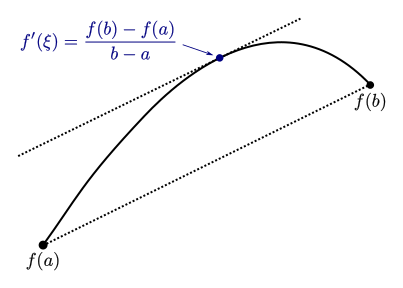
\includegraphics[width=0.5\textwidth]{mean_value_theorem}
    \end{figure*}
\end{example}

\begin{definition}
    We say that the Taylor series \textit{represents} the function $f$ at $x$
    if the Taylor series converges at that point, i.e. the remainder 
    tends to zero as $n \to \infty$.
\end{definition}

\begin{example}[1]
Back to $e^x$: $f(x) = e^x$, $c = 0$, $\xi_x$ is between $c$ and $x$.
\[
    e^x = \sum_{k=0}^n \frac{x^k}{k!} + \frac{e^{\xi_x}}{(n + 1)!} x^{n + 1}
\]

For any $x \in \mathbb{R}$ we find $s \in \mathbb{R}^{+}_{0}$ ($\mathbb{R}^{+}_{0}$ are
all real, positive numbers including 0)
so that $\abs{x} \le s$, and $\abs{\xi_x} \le s$ because $\xi_x$ is between $c$ and $x$.

\begin{figure*}[h]
    \centering
    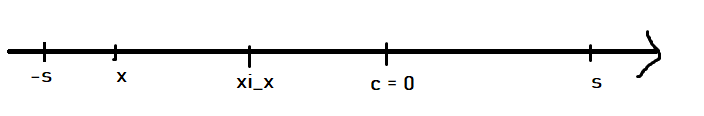
\includegraphics[width=0.7\textwidth]{some_axis}
\end{figure*}

Because $e^x$ is monotone increasing, we have $e^{\xi_x} \le e^s$, thus

\begin{align*}
    \lim_{n \to \infty} \abs{\frac{e^{\xi^x}}{(n+1)!} x^{n + 1}} \le
    \lim_{n \to \infty} \abs{\frac{e^s}{(n + 1)!}} s^{n + 1} = 
    e^s \lim_{n \to \infty} \frac{s^{n + 1}}{(n + 1)!} = 0
\end{align*}

Because $(n + 1)!$ will grow faster than any power of
$s \implies \lim_{n \to \infty} \abs{\frac{e^{\xi_x}}{(n + 1)!} x^{n + 1}} = 0$.

Thus $e^x$ is \textit{represented} by its Taylor series.
\end{example}

\begin{example}[2]
    \begin{align*}
        &
        f(x) = \log(1 + x),\ c = 0
        \\&
        f'(x) = \frac{1}{1+x} = (1 + x)^{-1}
        \\&
        f''(x) = -(1 + x)^{-2}
        \\&
        f'''(x) = +2(1 + x)^{-3}
        \\&
        f^{(k)}(x) = (-1)^{k + 1} (k - 1)! \frac{1}{(1 + x)^k}
    \end{align*}
\end{example}

So $f^{(k)}(0) = (-1)^{k - 1} (k - 1)!$ for $k \ge 1$, 
$f(0) = \log(1) = 0$.

Taylor series: 
\begin{align*}
    &
    f(x) = \sum_{k = 1}^n \frac{(-1)^{k - 1}}{k} x^k +
    \frac{(-1)^k}{n + 1} \frac{1}{(1 + \xi_x)^{n + 1}} \cdot x^{n + 1}
    \quad \Bigl(\frac{n!}{(n + 1)!} = \frac{1}{n + 1}\Bigr)
    \\&
    E_n(x) = \frac{(-1)^k}{n + 1} \frac{1}{(1 + \xi_x)^{n + 1}} \cdot x^{n + 1}
    \text{ --- the remainder}
\end{align*}
Question: for which $x$ does $\lim_{n \to \infty} E_n(x) = 0$?
\[
    \lim_{n \to \infty} E_n(x) =
    \lim_{n \to \infty} \frac{(-1)^n}{n + 1} \Bigl(\frac{x}{\xi_x + 1}\Bigr)^{n + 1}
    \text{ for } \xi_x \in (c, x)\ (c = 0)
\]
Such a limit converges to 0, if the fraction is less than 1.
\[
    0 < \frac{x}{\xi_x + 1} < 1 \Longleftrightarrow x < \xi_x + 1 \Longleftrightarrow
    x - \xi_x < 1 \text{ with } \xi_x \in (0, x) \Longleftrightarrow
    x \le 1
\]
\begin{consequence}
    $\lim_{n \to \infty} E_n(x) = 0$ if $0 < x \le 1$.
    This means that the Taylor series represents $\log(x + 1)$ for $x \in [0, 1]$.
    We can extend this to show $x \in (-1, 1]$.
\end{consequence}

\begin{example}[3]
    Let's compute $\cos(0.1)$. Let's approximate it with Taylor series with $c = 0$ (around zero).
    \[
        \cos(x) = 1 - \frac{x^2}{2} + \frac{x^4}{4!} - \frac{x^6}{6!} \pm \dots
        + \mathrm{remainder}
    \]
\end{example}
\begin{consequence}
    \[
        \abs{\cos(x) - \sum_{k=0}^n (-1)^k \frac{x^{2k}}{(2k!)}} =
        \abs{(-1)^{n + 1} \cos(\xi_x) \frac{x^{2(n + 1)}}{\bigl(2(n + 1)\bigr)!}} \le
        \frac{0.1^{2(n + 1)}}{2(n + 1)!} \underset{n \to \infty}{\longrightarrow} 0
    \]
\end{consequence}

\begin{center}
    \begin{tabular}{c | c | c}
        $n$ & Taylor polynomial & $\abs{\text{error}} \le$\\
        \hline
        0 & 1 & $\frac{(0.1)^2}{2} = 0.0005$\\
        1 & 0.995 & $\frac{0.0001}{24}$\\
        2 & 0.99500416 & $\frac{0.000001}{6!}$
    \end{tabular}
\end{center}

Error depends on choice of $\abs{x - c}$ and $n$.

\begin{example}[4]
    Compute $\log(2)$ using $f(x) = \log(x + 1)$
    \[
        \log(2) = 1 - \frac{1}{2} + \frac{1}{3} - \frac{1}{4} + \frac{1}{5} - \frac{1}{6} + \dots
    \]
    Keeping 8 terms (until $n = 8$) we get
    $\log(2) \approx 0.63452$, the actual solution is $\log(2) = 0.693147$. Not so accurate. Can we improve?

    We can use Taylor series of $\log\bigl(\frac{1 + x}{1 - x}\bigr)$ instead, 
    since $\log\bigl(\frac{1 + x}{1 - x}\bigr) = \log(1 + x) - \log(1 - x)$.
    We choose $x = \frac{1}{3}$ instead of $x = 1$.
    Since $x$ is closer to zero, both of the logarithms converge quicker.
    \[
        \biggl(\log\Bigl(\frac{1 + 1/3}{1 - 1/3}\Bigr) = \log(2) \biggr)
    \]
    We then get
    \[
        \log(2) = 2 \cdot \Bigl(\frac{1}{3} + \frac{1}{3^3 \cdot 5} + \dots\Bigr)
    \]
    We only need 4 terms to get
    $\log{2} \approx 0.69313$.
\end{example}

\begin{theorem}[Reformulation of Taylor's theorem]
    $f \in C^{n + 1}([a, b])$. We change $c$ to $x$ and the old $x$
    to $x + h$ from previous version $\implies$
    get for $x,\ x + h \in [a, b]$:
    \[
        f(x + h) = \sum_{k = 0}^n \frac{f^{(k)}(x)}{k!} h^k + 
        \frac{f^{(n + 1)}(\xi_x)}{(n + 1)!} h^{n + 1}
        \text{ where } \xi_x \in (x, x + h),\ h > 0
    \]

    We can write error term as 
    \[
        f(x + h) - \sum_{k=0}^n \frac{f^{(k)}(x)}{k!} h^k = \mathcal{O}(h^{n + 1})
    \]
\end{theorem}
\begin{remark}
    Let's recall what the $\mathcal{O}$-notation means.
    $a(h) = \mathcal{O}\bigl(b(h)\bigr)$ if $\exists c > 0$
    such that $\frac{a(j)}{b(j)} \le c$ as $h \to 0$.
    So, for $n = 1$ the error decreases with $h^2$ (quadratic convergence).\\
    $n = 2$: error decreases cubically, i.e. $h^3$, etc.
\end{remark}
\textbf{Summary of Taylor series:}
\begin{itemize}
    \item {
        Problem: Evaluate $f(x)$ with a given error bound.
    }
    \item {
        Required: $f \in \mathrm{C}^{n+1}$, values of derivatives $f^{(k)}(a)$.
    }
    \item {
        Check interval of convergence: does Taylor series expansion work?
    }
    \item {
        Estimate the maximum error for $n$ terms of the Taylor polynomial.
    }
    \item {
        Choose $n$, such that the error bound is low enough.
    }
    \item {
        Evaluate the Taylor polynomial.
    }
\end{itemize}

\newpage
\section{Number representation}

\subsection{Errors}
There are different error types:
\begin{enumerate}
    \item {
        An error in data (partly due to roundoff).
    }
    \item {
        Roundoff errors (during computation). For example,
        multiplication increases the amount of needed significant digits, and
        we can't store them all on a computer.
    }
    \item {
        Truncation error, that is inherent to numeric methods. For example,
        if we take a finite number of terms in our Taylor series.
    }
\end{enumerate}

\begin{definition}
    Let $\tilde{a}$ be an approximation of $a$. Then
    $\abs{\tilde{a} - a}$ is the \textit{absolute error}, and 
    $\abs{\frac{\tilde{a} - a}{a}}$ is the \textit{relative error}.
    The \textit{error bound} is the magnitude of admissable error.
\end{definition}
\begin{example}
    0.00123 with error $0.000004 = 0.4 \cdot 10^{-5}$.
    The error is below $\frac{1}{2} \cdot 10^{-t}$ with $t = 5$, so there's 5
    correct digits and 3 significant digits (the number of non-leading zeros).
\end{example}
\begin{example}
    0.00123 with error $0.000006 = 0.06 \cdot 10^{-4} > \frac{1}{2} \cdot 10^{-5}$.
    Only has 2 significant digits, because we have to round the error up.
\end{example}

\begin{theorem}
    In addition/subtraction the bounds for absolute errors are added,
    in multiplication/division the relative errors are added.
\end{theorem}
\begin{example}
    Solve $x^2 - 56x + 1 = 0$:
    \[
        x = 28 - \sqrt{783} \approx 28 - 27.982 \text{ (5 significant digits)} =
        0.018 \pm \frac{1}{2} \cdot 10^{-3}
    \]
    We end up with 2 significant digits in the answer, despite that we used to 
    have 5. That's why computers use floating point numbers, as
    leading zeros are bad.
\end{example}

\begin{definition}[Error propagation]
    If $y(x)$ is smooth, than the derivative $\abs{y(x)'}$
    can be interpreted as the sensitivity of $y(x)$ to errors in $x$.
    We can generalize this to functions of multiple variables:
    \[
        \abs{\Delta y} \le \sum \abs{\frac{\partial y}{\partial x_i}} \cdot \abs{\Delta x_i}
        \text{, where } \Delta y = \tilde{y} - y,\ \Delta x_i = \tilde{x_i} - x_i
    \]
    This is an empirical inequality that is only valid for small $\Delta x_i$.
    It is used a lot in physics.
\end{definition}

\subsection{Base representation}
\begin{definition}[Base representation]
    Every number $x \in \mathbb{N}$ can be written in the following form 
    as a unique expansion with respect to the base $b$, where
    $b \in \mathbb{N} \setminus \{1\}$:
    \begin{align*}
        &
        x = a_0 b^0 + a_1 b^1 + a_2 b^2 + \dots + a_n b_n = 
        \sum_{i=0}^n a_i b^i 
        \\&
        a \in \mathbb{N}_0,\ a_i < b,\ a_i \in \{0, \dots, b - 1\}
    \end{align*}
        
    Here $b$ is called the \textit{base}, $a_i$ are called the \textit{digits}.
    Humans usually use base 10. But, for example, computers
    can use base 2.

    For a real number $x \in \mathbb{R}$ we can write: 
    \[
        x = \sum_{i=0}^n a_i b^i + \sum_{i=1}^\infty a_{-i} b^{-i}
    \]
\end{definition}
\begin{example}
    $b=2:\ 1011 = 1 \cdot 2^0 + 1 \cdot 2^1 + 0 \cdot 2^2 + 1 \cdot 2^3 =
    (11)_{10}$
\end{example}
There are different algorithms that convert number systems.

\subsection{Euclid's algorithm}
Euclid's algorithm converts $(x)_{10}$ to $(y)_b$.
\begin{enumerate}%[label={\arabic*)}]
    \item {
        Input $(x)_{10}$.
    }
    \item {
        Determine the smallest $n$, such that $x < b^{n+1}$.
    }
    \item {
        For $i=n$ to $0$ do:
        \begin{align*}
            &
            a_i \coloneqq x\ \mathrm{div}\ b^{i} \text{ (integer division)}
            \\&
            x \coloneqq x\ \mathrm{mod}\ b^{i} \text{ (the remainder)}
        \end{align*}
    }
    \item {
        Output result $a_n a_{n-1} a_{n-2} \dots a_0 = (y)_b$.
    }
\end{enumerate}

\begin{example}
    \begin{enumerate}
        \item {
            $(x)_{10} = (13)_{10} \to (y)_2$
        }
        \item {
            $n = 3$ since $13 < 2^4$.
        }
        \item {
            \begin{align*}
                &
                i = 3:\ a_3 = 13 \ \mathrm{div}\ 2^3 = 1,\
                x = 13 \ \mathrm{mod}\ 2^3 = 5
                \\&
                i = 2:\ a_2 = 5 \ \mathrm{div}\ 2^2 = 1,\
                x = 5 \ \mathrm{mod}\ 2^2 = 1
                \\&
                i = 1:\ a_1 = 1 \ \mathrm{div}\ 2^1 = 0,\
                x = 1 \ \mathrm{mod}\ 2^1 = 1
                \\&
                i = 0:\ a_0 = 1 \ \mathrm{div}\ 2^0 = 1,\
                x = 1 \ \mathrm{mod}\ 2^0 = 0
            \end{align*}
        }
        \item {
             Output: $(1101)_2 = (13)_{10}$.
        }
    \end{enumerate}
\end{example}
Two problems of the Euclid's algorithm:
\begin{enumerate}
    \item {
        Step 2 is inefficient
    }
    \item {
        Division by large numbers can be problematic.
    }
\end{enumerate}

\subsection{Horner's scheme}
Horner's scheme is a more efficient algorithm. The idea is to represent
the number as follows:
\[
    (a_n a_{n - 1} \dots a_{0})_b = 
    a_0 + b\bigl(a_1 + b(a_2 + b(a_3 + \dots + b (a_n))) \dots \bigr)
\]
The algorithm is the following:
\begin{enumerate}
    \item {
        Input $(x)_{10}$.
    }
    \item {
        $i \coloneqq 0$.
    }
    \item {
        While $x > 0$ do:
        \begin{align*}
            &
            a_i \coloneqq x \ \mathrm{mod}\ b
            \\&
            x \coloneqq x \ \mathrm{div}\ b
            \\&
            i \coloneqq i + 1
        \end{align*}
    }
    \item {
        Output result $a_n a_{n-1} a_{n-2} \dots a_0 = (y)_b$.
    }
\end{enumerate}
\begin{remark}
    The algorithm is very similar to the Euclid's algorithm ---
    the difference is that we execute it in reverse. 
    We no longer have divisions by large numbers, and thus
    it runs faster.
\end{remark}

\textbf{General remarks:}
\begin{itemize}
    \item {
        A number with simple representation in one base 
        may be complicated to represent in another base.
        For example,
        $(0.1)_{10} = (0.0001100110011\dots)_2$.
    }
    \item {
        Base 2 is called \textit{binary},
        base 8 is \textit{octal},
        base 16 is \textit{hexadecimal}.
    }
    \item {
        To convert from a base $b$
        to base $10$ we can just perform the following computation:
        \[
            (42)_8 = 4 \cdot 8^1 + 2 \cdot 8^0 = (34)_{10}
        \]
    }
    \item {
        Conversion $2$ and $8$. $8=2^3$:
        three consecutive bits represent one octal digit, e.g.
        \[ (551.624)_8 = (101 101 001.110 010 100)_2 \]
    }
    \item {
        Conversion $2$ and $16=2^4$: just four bits to one hexadecimal digit. 
    }
    \item {
        Horner's scheme algorithm does not need estimate of $n$
        and does not divide by large numbers.
    }
    \item {
        It is applicable to real numbers, but one needs a critireon to stop
        if the representation with the new base is infinite.
    }
    \item {
        On computers we only have finite precision
        (the number of digits/bits).
    }
\end{itemize}
\begin{definition}[Measurable space]
    A \textit{measurable space} is a tuple $(X, \mathcal{A})$, where:
    \begin{enumerate}
        \item {
            $X$ is a set.
        }
        \item {
            $\mathcal{A}$ is a $\sigma$-algebra on $X$.
        }
    \end{enumerate}
\end{definition}

\begin{definition}[Measure space]
    A \textit{measure space} is a triple $(X, \mathcal{A}, \mu)$, where:
    \begin{enumerate}
        \item {
            $X$ is a set.
        }
        \item {
            $\mathcal{A}$ is a $\sigma$-algebra on $X$.
        }
        \item {
            $\mu$ is a measure on $(X, \mathcal{A})$.
        }
    \end{enumerate}
\end{definition}

\begin{example}[1]
    $\{\emptyset, X\}$ is a $\sigma$-algebra. Any $\mu$, such that
    $\mu(\emptyset) = 0$ and $\mu(X) \ge 0$ will be a measure.
\end{example}
\begin{example}[2]
    $2^X$ is a $\sigma$-algebra. We can have the following measures:
    \begin{enumerate}[label=\alph*)]
        \item {
            $\mu(E) = \abs{E}$ is called a \textit{counting measure}.
            Here $\abs{E}$ denotes the cardinality of $E$ (number of elements in $E$).
        }
        \item {
            $\delta$-measure (also called Dirac measure):
            \[
                \mu(E) = \begin{cases}
                    1, &0 \in E\\
                    0, &\text{otherwise}
                \end{cases}
            \]
        }
    \end{enumerate}
\end{example}

\subsection{Continuity of measure}

\begin{definition}
    A countable collection of sets $\{E_k\}_{k=1}^\infty$ is called
    \textit{ascending} if $E_k \subset E_{k+1}$.
\end{definition}
\begin{definition}
    A countable collection of sets $\{E_k\}_{k=1}^\infty$ is called
    \textit{descending} if $E_k \supset E_{k+1}$.
\end{definition}

\begin{theorem}[Continuity of measure]
    \label{the:continuityOfMeasure}
    \item{} % Newline hack
    \begin{enumerate}
        \item {
            If $\{A_k\}_{k=1}^\infty \subset \mathcal{A}$ and the sequence is ascending,
            then
            \[
                \mu\Bigl(\bigcup_{k=1}^\infty A_k\Bigr) = \lim_{k \to \infty} \mu(A_k)
            \]
        }
        \item {
            If $\{B_k\}_{k=1}^\infty \subset \mathcal{A}$, the sequence is descending and $\mu(B_1) < \infty$,
            then
            \[
                \mu\Bigl(\bigcap_{k=1}^\infty B_k\Bigr) = \lim_{k \to \infty} \mu(B_k)
            \]
        }
    \end{enumerate}
\end{theorem}
\begin{proof}
    \begin{enumerate}
        \item {
            Let $C_k \coloneqq A_k \setminus A_{k-1}$. Then we have:

            \begin{figure*}[h]
                \centering
                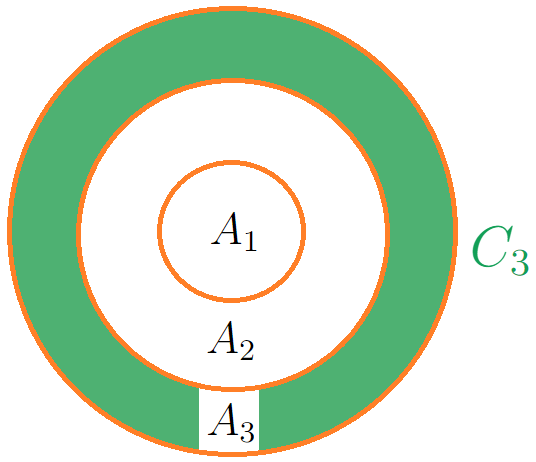
\includegraphics[width=0.3\textwidth]{a1a2a3}
            \end{figure*}

            \[
                \mu\Bigl(\bigcup_{k=1}^\infty A_k\Bigr) =
                \mu\Bigl(\bigsqcup_{k=1}^\infty C_k\Bigr) =
                \sum_{k=1}^\infty \mu(C_k) =
                \lim_{n \to \infty} \sum_{k=1}^n \mu(C_k) = \lim_{n \to \infty} \mu(A_n)
            \]
        }
        \item {
            Let $D_k \coloneqq B_1 \setminus B_k$. 
            Since $B_k$ is descending, it follows that $D_k$ is an ascending sequence. Then from the part 1 of the theorem it follows that:
            \begin{align*}
                &
                \mu\Bigl(\bigcup_{k=1}^\infty D_k\Bigr) = \lim_{k \to \infty} \mu(D_k)
                \qquad
                \bigcup_{k=1}^\infty D_k = B_1 \setminus \bigcap_{k=1}^\infty B_k
                \\&
                \mu\Bigl(B_1 \setminus \bigcap_{k=1}^\infty B_k\Bigr) =
                \lim_{k \to \infty}\bigl(\mu(B_1) - \mu(B_k)\bigr) =
                \mu(B_1) - \lim_{k \to \infty} \mu(B_k)
                \\&
                \mu\Bigl(B_1 \setminus \bigcap_{k=1}^\infty B_k\Bigr) =
                \mu(B_1) - \mu\Bigl(\bigcap_{k=1}^\infty B_k\Bigr) \implies
                \mu\Bigl(\bigcap_{k=1}^\infty B_k\Bigr) = \lim_{k \to \infty} \mu(B_k)
            \end{align*}
        }
    \end{enumerate}    
\end{proof}

\begin{definition}
    We say that a statement (property) holds for \textit{almost all} $x \in X$
    \textit{with respect to a measure $\mu$}, if
    $\exists N \in \mathcal{A}$, such that $\mu(N) = 0$ and the statement (property)
    holds for all $x \in X \setminus N$.
\end{definition}
\begin{lemma}[Borel–Cantelli]
    Let $(X, \mathcal{A}, \mu)$ be a measure space. Let
    $\{E_k\}_{k=1}^\infty \subset \mathcal{A}$ and $\sum_{k=1}^\infty \mu(E_k) < \infty$.
    Then \textit{almost all} $x \in X$ belong to at most finitely many $E_k$.
\end{lemma}
\begin{proof}
    Let $B_n = \cup_{k=n}^\infty E_k$. It's easy to see that $B_k$ is a descending measure.
    At the same time,
    \[ \mu(B_1) = \mu\Bigl(\bigcup_{k=1}^\infty E_k\Bigr) \le \sum_{k=1}^\infty \mu(E_k) < \infty \]
    By definition of $B_n$, $\cap_{n=1}^\infty B_n$ contains all the points
    that are contained in infinitely many $E_k$'s. But, by \hyperref[the:continuityOfMeasure]{continuity of measure} 
    for $\{B_n\}_{n=1}^\infty$ we have:
    \[ 
        \mu\Bigl(\bigcap_{n=1}^\infty B_n\Bigr) =
        \lim_{n \to \infty} \mu(B_n) =
        \lim_{n \to \infty} \Bigl(\bigcup_{k=n}^\infty E_k\Bigr) \le
        \lim_{n \to \infty} \sum_{k=n}^\infty \mu(E_k) = 0
    \]
\end{proof}

\subsection{How large is the Lebesgue $\sigma$-algebra $\mathcal{M}$?}
\begin{proposition}
    \label{prop:intervalsAreMeasurable}
    Every interval is Lebesgue-measurable.
\end{proposition}
\begin{proof}
    Proof idea:
    \[ 
        E \in \mathcal{M} \Longleftrightarrow 
        \forall A: m(A) = m(A \cap E) + m(A \cap E^C)
    \]
    Assume $E = (-\infty, a)$. If we prove that such intervals lie in $\mathcal{M}$, 
    then we'll prove everything (since $\mathcal{M}$ is a $\sigma$-algebra).
    We already have $m(A) \le m(A \cap E) + m(A \cap E^C)$ from \hyperref[the:countableSubadditivity]{countable subadditivity}.

    Let's assume $a \not\in A$ (since removing one point does not change the measure).
    Every cover of $A$ can be split into two covers with the same sum of interval lengths: of
    $A \cap (-\infty, a)$ and $A \cap (a, +\infty)$. Every interval in those
    covers, that contains $a$, can be split into two. Therefore,
    from the \hyperref[def:lebesgueOuterMeasure]{definition of Lebesgue measure}, 
    $m(A) \ge m(A \cap E) + m(A \cap E^C)$, so we've proved the inequality in both sides.
\end{proof}
\begin{definition}
    For any $\mathcal{X} \in 2^\mathbb{R}$ let $\mathcal{A}(\mathcal{X})$
    be the smallest $\sigma$-algebra containing $\mathcal{X}$.
\end{definition}

\begin{lemma}
    $\mathcal{A}(\mathcal{X})$ always exists and is the intersection of all $\sigma$-algebras
    containing $\mathcal{X}$.
\end{lemma}
\begin{proof}
    We have to prove that if we intersect a bunch $\sigma$-algebras, we still get a 
    $\sigma$-algebra.
    \begin{enumerate}
        \item {
            Such an intersection is closed under complements:
            if a set belongs to the intersection of $\sigma$-algebras,
            then it belongs to each of the $\sigma$-algebras, 
            then its complement belongs to each of the $\sigma$-algebras,
            and thus its complement belongs to the intersection of 
            $\sigma$-algebras.
        }
        \item {
            In a similar way, such an intersection is closed under countable unions:
            if a number of sets all belong to the intersection of $\sigma$-algebras,
            then they all belong to each of the $\sigma$-algebras, 
            then their countable union belongs to each of the $\sigma$-algebras,
            and their countable union belongs to the intersection of 
            $\sigma$-algebras.
        }
    \end{enumerate}
\end{proof}

\begin{remark}
    We can try to construct $\mathcal{A}(\mathcal{X})$ in a different way.
    Say, $\mathcal{X}$ is not a $\sigma$-algebra. Let's enlarge it:
    first by including all the complements. Then let's enlarge it
    by all countable unions. Let's call such a set $\mathcal{X}_1$.
    But after such operation, $\mathcal{X}_1$ may be non-closed under complements.
    So we repeat such a procedure.

    And, in general: $\mathcal{X}_{n + 1}$ is obtained from $\mathcal{X}_n$
    is obtained by including into $\mathcal{X}_n$ all complements of the 
    sets from $\mathcal{X}_n$ and then including all countable unions of the obtained sets.

    \begin{figure*}[h]
        \centering
        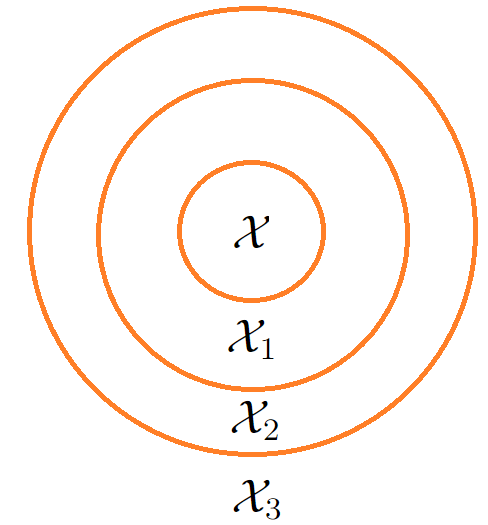
\includegraphics[width=0.3\textwidth]{some_circles}
    \end{figure*}

    It is tempting to think that $\cup_{1}^\infty \mathcal{X}_i$ is $\mathcal{A}(\mathcal{X})$.
    Is it true? No, not necessarily.
    If the sequence $\{\mathcal{X}_i\}$ eventually stabilizes, then such a construction works.
    Let's now assume that every next $\mathcal{X}_i$ is larger than the previous one.
    Then we can take $A$ from $\mathcal{X}$, $A_1$ from $\mathcal{X}_1 \setminus \mathcal{X}$,
    $A_2$ from $\mathcal{X}_2 \setminus \mathcal{X}_1$, and so on.

    Now let's look at $\cup_{1}^\infty A_i$. As a countable union, it must be contained
    in $\mathcal{A}(\mathcal{X}) = \cup_{1}^\infty \mathcal{X}_i$, thus, there exist an $n$, such that
    $\cup_{1}^\infty A_i \in \mathcal{X}_n$. But $A_{n+1} \in \mathcal{X}_{n+1} \setminus \mathcal{X}_n$?!
\end{remark}

\begin{definition}[Topological space]
    A \textit{topological space} is a set $X$ and a collection
    of subsets $O$ of $X$ (called \textit{open sets}), such that $\emptyset, X \in O$, and:
    \begin{enumerate}
        \item {
            A union of (possibly infinitely many) sets from $O$
            is in $O$.
        }
        \item {
            The intersection of finitely many sets from $O$
            is in $O$.
        }
    \end{enumerate}
    The complements of open sets are called \textit{closed sets}.
\end{definition}

\begin{definition}
    A function $f : X \to Y$ between two topological spaces is \textit{continuous} if
    the preimage of every open set is open.
\end{definition}
\begin{remark}
    It is possible to check that for $\mathbb{R}$ this definition is
    equivalent to the usual one.
\end{remark}

\begin{definition}[Borel $\sigma$-algebra]
    For a topological space $X$ its \textit{Borel $\sigma$-algebra $\mathcal{B}_X$}
    is the smallest $\sigma$-algebra on $X$ that contains all open sets. 
\end{definition}
\begin{remark}
    If it's obvious from the context which set we are talking about,
    we will just write $\mathcal{B}$ (without a subscript).
\end{remark}

\begin{theorem}
    $\mathcal{B}_\mathbb{R} \subset \mathcal{M}$ (all of the sets in $\mathcal{B}_\mathbb{R}$ are measurable).
\end{theorem}
\begin{proposition}
    \label{prop:bIsSmallestSigmaAlgebra}
    $\mathcal{B}$ is the smallest $\sigma$-algebra that contains all open intervals.
\end{proposition}
If we prove the proposition, the theorem will follow easily.
We know that \hyperref[prop:intervalsAreMeasurable]{all the intervals are Lebesgue-measurable}.
We know that the Lebesgue-measurable sets ($\mathcal{M}$) 
\hyperref[the:mIsSigmaAlgebra]{are a $\sigma$-algebra}.
Thus, if we take the smallest $\sigma$-algebra that contains all open intervals,
it will be a subset of $\mathcal{M}$.
\begin{proof}[Proof of Proposition~\ref{prop:bIsSmallestSigmaAlgebra}]
    We will prove that every open set $O \subset \mathbb{R}$ is a finite or
    countable union of open intervals.

    For every point $x \in O$ let $I_x$ be the largest open interval, such that
    $x \in I_x$ and $I_x \subset O$.
    It exists as a union of all such intervals. Since $O$ is open, 
    $x$ lies in $O$ with an open neighborhood,
    thus, $I_x$ is non-empty.
    \[
        \forall x \in O: x \in I_x \implies
        O = \bigcup_{x \in O} I_x
    \]
    Let's prove that $I_x \cap I_y \ne \emptyset \implies I_x = I_y$. If the intervals
    around $x$ and $y$ intersect, then $I_x \cup I_y$ is an interval as well, and
    $I_x \cup I_y \in O$ as $I_x \in O$ and $I_y \in O$. Since $I_x$ and $I_y$ are the largest such intervals, it follows that
    $I_x = I_x \cup I_y = I_y$.

    Let's say that two points $x$ and $y$ are equivalent if $I_x = I_y$.
    Since there's a lot of same intervals in $O = \cup_{x \in O} I_x$,
    we can take just a single point from every equivalence class and still get $O$ 
    as a union. Particularly, every open interval contains at least one rational point
    (as rational numbers are dense). Therefore, there's a rational point
    in every equivalence class.
    Thus,
    \[ O = \bigcup_{x \in O \cap \mathbb{Q}} I_x \]
    Since the set of rational numbers is countable, we have represented $O$
    as a countable union of open intervals, which is what we wanted.
\end{proof}

\begin{remark}
    A topological space is called \textit{separable}, if it contains a 
    countable dense subset.
\end{remark}
\begin{remark}
    We have proved that the Lebesgue measure exists on $\mathcal{B}_\mathbb{R}$,
    so we have a lot of measurable sets.
\end{remark}
\begin{remark}
    The Lebesgue measure can be generalized to $\mathbb{R}^n$.
\end{remark}
GE can be used whenever the pivots don't vanish.
\begin{example}
    \[
    \begin{cases}
        x_1 + x_2 + x_3 = 1\\
        x_1 + x_2 + 2x_3 = 2\\
        x_1 + 2x_2 + 2x_3 = 1
    \end{cases} \implies
    \begin{cases}
        x_1 = 1\\ x_2 = -1 \\ x_3 = 1
    \end{cases}
\]

But addition of rows will give us:
\[
    \begin{cases}
        x_3 = 1 \text{ -- here we have a missing pivot}\\
        x_2 + x_3 = 0
    \end{cases}
    \qquad
    \left(\begin{array}{ccc|c}
        0 & 0 & 1 & 1\\
        0 & 1 & 1 & 0\\
        1 & 2 & 2 & 1
    \end{array}
    \right)
\]
\end{example}

We already get into trouble with
very small pivot elements.
\begin{example}
    Let $\varepsilon > 0$ and consider
    \[
        \begin{cases}
            \varepsilon x_1 + x_2 = 1\\
            x_1 + x_2 = 2
        \end{cases}
        \Longleftrightarrow
        \begin{pmatrix}
            2 & 1\\
            1 & 1
        \end{pmatrix}
        \vec{x} = \begin{pmatrix}
            1 \\ 2
        \end{pmatrix}
    \]
    For $\varepsilon \ll 1$, the actual solution is $x_1 \approx x_2 \approx 1$.
    However, GE yields
    \[
        x_2 = \frac{2 - \frac{1}{\varepsilon}}{1 - \frac{1}{\varepsilon}}
        \overset{\varepsilon \ll 1}{\approx}
        \frac{-\frac{1}{\varepsilon}}{-\frac{1}{\varepsilon}} = 1
    \] 
    WIth finite precision we will get through backward substitution:
    $x_2 = 1$ and $x_1 = \frac{1 - x_2}{\varepsilon} = 0$ which is wrong.
    The pivot is too small. But change order of equations.
    \[
        \begin{cases}
            x_1 + x_2 = 2\\
            \varepsilon x_1 + x_2 = 1
        \end{cases}
        \overset{\text{GE}}{\implies}
        \begin{cases}
            x_2 = \frac{1 - 2\varepsilon}{1 - \varepsilon}\\
            x_1 = 2 - x_2
        \end{cases}
    \]
    Now the answer is correct. The reason why the first one was incorrect is
    error amplification of $x_2$ by multiplication.
    $\frac{1}{\varepsilon}$ leads in the first case to a wrong result.
\end{example}

\subsection{Scaled partial pivoting}
\begin{definition}
    \textit{Pivoting} means that the pivot element is chosen 
    appropriately, and not just row by row.
\end{definition}
\begin{definition}
    \textit{Partial pivoting} means we will reorder rows
    (not columns, otherwise it would be full pivoting).
\end{definition}
\begin{definition}
    \textit{Scaled} means we look for best \textit{relative} pivot,
    i.e. best ratio between pivot element and maximal entry of row
    (all in absolute values).
\end{definition}
\begin{remark}
    This will lead to minimal error propagation.
\end{remark}

The algorithm:
\begin{enumerate}
    \item {
        Input $A \in \mathbb{R}^{n \times n},\ b \in \mathbb{R}^m$.
    }
    \item {
        Find maximal absolute values of entries in rows
        $s \in \mathbb{R}^n$, such that $s_i = \max_{j=1}^n \abs{a_{ij}}$.

        Forward elimination:
    }
    \item {
        For $k = 1, \dots, n - 1$  (for all pivot rows).
    }
    \item {
        \hspace*{0.5cm} For $i = k, \dots, n$ (for all rows below pivot row)\\
        \hspace*{1cm} compute $\abs{\frac{a_{ik}}{s_i}}$.
    }
    \item[$\overline{4}$.] {
        \hspace*{0.5cm} End for.
    }
    \item {
        \hspace*{0.5cm} Find row with the largest relative pivot element, 
        name it row $j$.
    }
    \item {
        \hspace*{0.5cm} Swap $k$ with $j$.
    }
    \item {
        \hspace*{0.5cm} Swap entries $k$ and $j$ in vector $s$.
    }
    \item {
        \hspace*{0.5cm} Do skip of forward elimination in row $k$.
    }
    \item[$\overline{3}$.] {
        End for.
    }
\end{enumerate}
Backward substitution is done as before, but with updated order.
\begin{example}
    \[
        \left[
        \begin{array}{cccc|c}
            3 & -13 & 9 & 3 & -19\\
            -6 & 4 & 1 & -18 & -32\\
            6 & -2 & 2 & 4 & 16\\
            -12 & -8 & 6 & 10 & 26
        \end{array}
        \right]
    \]
    Initial $s = (13, 18, 6, 12)$.
    Iterations:
    \begin{enumerate}
        \item {
            \begin{itemize}
                \item {
                    Relative pivots:
                    \[
                        \Bigl(
                            \frac{3}{13}, \frac{6}{18},
                            \frac{6}{6}, \frac{12}{12}
                        \Bigr) =
                        \biggl(\abs{\frac{a_{ik}}{s_i}}\biggr)
                    \]
                }
                \item {
                    Rows 3 and 4 have pivot 1 greater than all others.
                    Select for swapping rows 1 and 3.
                    \[
                        \left[\begin{array}{cccc|c}
                            6 & -2 & 2 & 4 & 16\\
                            -6 & 4 & 1 & -18 & -32\\
                            3 & -13 & 9 & 3 & -19\\
                            12 & -8 & 6 & 10 & 26
                        \end{array}\right]
                    \]
                }
                \item {
                    Swap entries $3 \leftrightarrow 1$ in $s$:
                    $(6, 18, 13, 12)$.
                }
                \item {
                    Forward elimination step (like in GE):
                    \[
                        \left[\begin{array}{cccc|c}
                            6 & -2 & 2 & 4 & 16\\
                            0 & 2 & 3 & -14 & -18\\
                            0 & -12 & 8 & 1 & -27\\
                            0 & -4 & 2 & 2 & -6
                        \end{array}\right]
                    \]
                }
            \end{itemize}
        }
        \item {
            On the second iterations, $k = 2$.
            \begin{itemize}
                \item {
                    Relative pivots (we don't care about the first row anymore, so just three rows left):
                    \[ \biggl( \abs{\frac{2}{18}}, \abs{\frac{12}{13}}, \frac{4}{12} \biggr) \]
                    The second ratio is the largest, and it corresponds to the third row.
                }
                \item {
                    So, we swap row 3 with row $k = 2$.
                }
                \item {
                    Swap entries in $s$.
                }
                \item {
                    Forward elimination. Then backward substitution
                    on updated matrix as before.
                }
            \end{itemize}
        }
    \end{enumerate}
\end{example}

Remarks:
\begin{itemize}
    \item {
        In efficient implementations, the step of row swapping can be omitted, just 
        a permutation vector $l$ needs to be stored to keep track of matrix
        rearrangements.
        This will result in "echelon form" that will look like e.g.
        \[
            \begin{array}{c}
                2\ \to\\
                4\ \to\\
                1\ \to\\
                3\ \to
            \end{array}
            \left[\begin{array}{cccc|c}
                0 & * & * & * & *\\
                0 & 0 & 0 & * & *\\
                * & * & * & * & *\\
                0 & 0 & * & * & *
            \end{array}\right]
        \]
    }
    \item {
        GE with scaled partial pivoting always works when matrix is invertible, i.e.
        there exists a $A^{-1}$, such that $A A^{-1} = I$.
    
        It will fail for a singular (i.e. not invertible) matrix,
        because eventually a division by 0 will occur.
    }
    \item {
        Doing Gaussian elimination has computational complexity
        of $\mathcal{O}(n^3)$, because we have three nested for-loops.
        Cubic behaviour $n^3$ is problematic for large $n$!
    }
    \item {
        Traditionally, only the multiplication/division operations
        were counted in the number of operations $C$.
        (Since addition is very cheap).
        On present-day hardware, however, the costs are nearly as ``cheap''
        as addition or subtraction.
    }
    \item { 
        We are missing costs due to exchange with memory.
        Therefore, estimates of time complexity and reality may
        diverge substantially. 
    }
    \item {
        Backward substitution has order $n^2$, which does not affect the general 
        estimate of $n^3$.
    }
    \item {
        Scaled partial pivoting leads to an increase in cost, but order stays $n^3$.
    }
\end{itemize}
\subsection{Banded systems}
\begin{definition}
    An equation system is called \textit{banded}
    if $a_{ij} \ne 0, \abs{i - j} \le k < n$, i.e.
    non-zero entries are arranged around the diagonal.
    
\end{definition}
\begin{example}
    \[
        \begin{pmatrix}
            * & * & 0 & 0 & 0 & 0\\ 
            * & * & * & 0 & 0 & 0\\ 
            0 & * & * & * & 0 & 0\\ 
            0 & 0 & * & * & * & 0\\ 
            0 & 0 & 0 & * & * & *\\ 
            0 & 0 & 0 & 0 & * & *
        \end{pmatrix}
    \]
    Is a 3-banded system with $k = 1$.
\end{example}
\begin{remark}
    Banded systems can occur in image filtering and many other problems.
\end{remark}
\begin{remark}
    Solving Gaussian Elimination is $\mathcal{O}(n^3)$, banded systems: $\mathcal{O}(n)$.
\end{remark}
\begin{remark}
    The case of $k = 1$ is called triagonal or three diagonal.
\end{remark}

\textbf{General remarks:}
\begin{itemize}
    \item {
        A nonsingular matrix is called \textit{regular}, it has full rank
        and has an inverse.
    }
    \item {
        A square matrix is nonsingular if the determinant $\ne 0$.
    }
    \item {
        If the matrix is singular, GE (both versions) will lead to division by zero
        (zero pivots) at some stage, or a floating point exception.
        You don't have to check for this explicitely: once you get an exception, 
        you know the matrix is singular.
    }
    \item {
        Errors. If we're trying to solve $Ax = b$ and we found the solution
        $x = \tilde{x}$, then the error is $r = A\tilde{x} - b$.

        If $\norm{r}$ is large due to rounding, we call the matrix \textit{ill-conditioned}.
    }
\end{itemize}

\subsection{LU Decomposition}
\begin{itemize}
    \item {
        In many applications the same linear system has to be solved for different right
        hand sides.
    }
    \item {
        If you know the inverse, you can simply apply it to the right hand side:
        \begin{align*}
            &
            x_1, x_2, x_3 \in \mathbb{R}^n, A \in \mathbb{R}^{n \times n}
            \\&
            Ax_1 = b_1,\ Ax_2 = b_2, Ax_3 = b_3
            \\&
            x_1 = A^{-1} b_1,\ x_2 = A^{-1} b_2,\ x_3 = A^{-1} b_3
        \end{align*}
    }
    \item {
        We want to store the operations of GE
        and backward substitution in a convenient way,
        so we can easily solve for different $b$.
    }
    \item {
        The key operation is: all the row operations
        of GE can be formulated as linear operators (which can be represented as matrices).
        
        In forward \textit{elimination}, i.e. adding a multiple of an upper row to a lkower row, 
        the matrices are lower-triangular.
    }
\end{itemize}

\begin{example}
    \[M_1 = \begin{bmatrix}
        1 & 0 & 0 & 0\\
        -2 & 1 & 0 & 0\\
        -\frac{1}{2} & 0 & 1 & 0\\
        1 & 0 & 0 & 1
    \end{bmatrix}\]
    $M_1 A$ does the following:
    \begin{itemize}
        \item {
            Leave the first row as is.
        }
        \item {
            Subtract 2 row 1 from row 2.
        }
        \item {
            Subtract $\frac{1}{2}$ row 1 from row 3.
        }
        \item {
            Adds row 1 to row 4.
        }
    \end{itemize}
    Reducing echelon form in 3 steps by $M_3 M_2 M_1 A$
    and we get new system
    \[ Ax = b \Longleftrightarrow M_3 M_2 M_1 A = M_3 M_2 M_1 b
    \text{, where $M_3 M_2 M_1$ is an upper-triangular matrix} \]
    Previous example gives us (GE without partial pivot):
    \[
        M_1 = \begin{bmatrix}
            1 & 0 & 0 & 0\\
            -2 & 1 & 0 & 0\\
            -1/2 & 0 & 1 & 0\\
            1 & 0 & 0 & 1
        \end{bmatrix},\quad
        M_2 = \begin{bmatrix}
            1 & 0 & 0 & 0\\
            0 & 1 & 0 & 0\\
            0 & -3 & 1 & 0\\
            0 & 1/2 & 0 & 1
        \end{bmatrix},\quad
        M_3 = \begin{bmatrix}
            1 & 0 & 0 & 0\\
            0 & 1 & 0 & 0\\
            0 & 0 & 1 & 0\\
            0 & 0 & -2 & 1
        \end{bmatrix}
    \]
\end{example}
\begin{remark}
    \mbox{}
    \begin{itemize}
        \item {
            Product of lower triangular matrices is a lower triangular matrix.
        }
        \item {
            Inverse of a lower triangular matrix is a lower triangular matrix.
        }
    \end{itemize}
\end{remark}
\textbf{Summary}:
If $M_3 M_2 M_1 A = U$, where $U$ --- upper-triangular matrix, then
\[ A = (M_3 M_2 M_1)^{-1} U = M_1^{-1} M_2^{-1} M_3^{-1} U = LU \]

Let's formulate a theorem to somewhat formalize things.
\begin{theorem}
    Let $A \in \mathbb{R}^{n \times n}$ be \textit{invertible}. Then there exists
    a decomposition $LU = A$ with $L$ --- a lower triangular matrix, and $U$ --- 
    upper triangular, $L, U \in \mathbb{R}^{n \times n}$ and
    $L = M_1^{-1} M_2^{-1} \dots M_{n-1}^{-1}$,
    where $M_i$ is the matrix describing step $i$ of forward elimination of GE.
    $U$ is upper-triangular-matrix (echelon form).
    \[U = M_{n-1} M_{n-2} \dots M_1 A \]
\end{theorem}
\begin{remark}
    LU can be done with pivoting, called LUP decomposition. There will be other matricies
    involved which swap rows.
\end{remark}
\begin{example}
    \begin{align*}
        A &= \begin{bmatrix}
            6 & -2 & 2 & 4\\
            -12 & -8 & 6 & 10\\
            3 & -13 & 9 & 3\\
            -6 & 4 & 1 & -18
        \end{bmatrix}
        \\
        U &= \begin{bmatrix}
            6 & -2 & 2 & 4\\
            0 & -4 & 2 & 2\\
            0 & 0 & 2 & -5\\
            0 & 0 & 0 & 3
        \end{bmatrix}
        \\
        M_1 &= \begin{bmatrix}
            1 & 0 & 0 & 0\\
            -2 & 1 & 0 & 0\\
            -\frac{1}{2} & 0 & 1 & 0\\
            1 & 0 & 0 & 1
        \end{bmatrix}
        \\
        M_1^{-1} &= \begin{bmatrix}
            1 & 0 & 0 & 0\\
            2 & 1 & 0 & 0\\
            \frac{1}{2} & 0 & 1 & 0\\
            -1 & 0 & 0 & 1
        \end{bmatrix} \text{ (notice the sign change)}
    \end{align*}
    I.e. $M_1^{-1}$ is an opposite operation to $M_1$:
    subtraction $\to$ addition, addition $\to$ subtraction.
    \[
        \implies L = M_1^{-1} M_2^{-2} M_3^{-1} =
        \begin{bmatrix}
            1 & 0 & 0 & 0\\
            2 & 1 & 0 & 0\\
            1/2 & 3 & 1 & 0\\
            -1 & -1/2 & 2 & 1
        \end{bmatrix}
    \]
    Finally, for solving $Ax = b$ we see
    $Ax = b \Longleftrightarrow LUx = b$.
    We do a substitution $y \coloneqq UX$.
    We solve for $y$ first, which is easy, since $L$ is triangular.
    Once we have $y$, we can solve $Ux = y$ for $x$ via backwardd substitution.
\end{example}

Remarks:
\begin{itemize}
    \item {
        LU has same complexity as GE ($\mathcal{O}(n^3)$).
    }
    \item {
        Any of the two substitution steps are $\mathcal{O}(n^2)$.
    }
\end{itemize}

\subsection{Cholesky decomposition}
When $A \in \mathbb{R}^{n \times n}$ is symmetric and positive definite,
we can use Cholesky decomposition.

\begin{definition}
    $B \in \mathbb{R}^{n \times n}$ is positive definite if and only if:
    \begin{enumerate}
        \item {
            All eigenvalues are greater than 0.
        }
        \item {
            $v \cdot Bv > 0$ when $v \ne 0$.

            $v \cdot Bv > 0 \Longleftrightarrow v = 0$.
        }
    \end{enumerate}
\end{definition}
\pagebreak
\subsection{Cholesky decomposition}

\begin{definition}
    $B \in \mathbb{R}^{n \times n}$ is positive definite if and only if:
    \begin{enumerate}
        \item {
            All eigenvalues are greater than 0.
        }
        \item {
            $v \cdot Bv > 0$ when $v \ne 0$.

            $v \cdot Bv = 0 \Longleftrightarrow v = 0$.
        }
    \end{enumerate}
\end{definition}

\begin{statement}
    When $B$ is symmetric and real, then all of the eigenvalues of it are real numbers.
\end{statement}

\begin{definition}[Cholesky decomposition]
    When $A \in \mathbb{R}^{n \times n}$ is symmetric and positive definite,
    then $A$ can be decomposed in the following form:
    \[ A = LDL^\intercal \]
    where:
    \begin{itemize}
        \item {
            $L$ is lower triangular, $a_{ii} = 1$, $i = 1, \dots, n$.
        }
        \item {
            $D$ is diagonal matrix with positive entries
        }
        \item {
            Because $D$ has only positive entries, we can we can 
            take the "square root" of it, i.e. find $\tilde{D}$, such that
            $D = \tilde{D} \tilde{D}$.
            So,
            \[ A = L D L^\intercal = (L\tilde{D}) (\tilde{D} L^T) = \tilde{L} \tilde{L}^\intercal \]
            Here $\tilde{D} = D$ as $D$ is diagonal.
        }
    \end{itemize}
\end{definition}

With such a decomposition, we can solve $Ax = b$ as
$Ax = \tilde{L} \tilde{L}^\intercal x = b$, where
$\tilde{L}$ is lower-triangular and $\tilde{L}^\intercal$ is upper-triangular.

The advantage from LU decomp is that we only need to save one matrix,
and forward substitution of the same kind will be carried out twice (so the matrix
will already be in cache).

The complexity if $\mathcal{O}(n^3)$, but compared to LU approximately half the operations
are needed.

How to compute $\widetilde{L}$? Let's suppose
\[
    \tilde{L} = \begin{bmatrix}
        l_{11} & 0 & \dots & 0\\
        l_{21}  & l_{22} & \dots & 0\\
        \vdots & \vdots & \ddots & \ddots\\
        l_{n1} & \dots & \dots & l_{nn}
    \end{bmatrix}
\] 
Then
\[
    \begin{bmatrix}
        a_{11} & \dots & a_{1n}\\
        \vdots & \ddots & \vdots\\
        a_{n1} & \dots & a_{nn}
    \end{bmatrix} =
    \begin{bmatrix}
        l_{11} & \dots & 0\\
        \vdots & \ddots & \vdots\\
        l_{n1} & \dots & l_{nn}
    \end{bmatrix} \cdot
    \begin{bmatrix}
        l_{11} & \dots & l_{n1}\\
        \vdots & \ddots & \vdots\\
        0 & \dots & l_{nn}
    \end{bmatrix}
\]
Then it follows by the formula of matrix multiplications:
\[ a_{ij} = \sum_{k=1}^n l_{ik} l_{jk} \]
Since a lot of entries in $\tilde{L}$ are zeros, actually
\[ a_{ij} = \sum_{k = 1}^j l_{ik} l_{jk},\ i \ge j \]
We only write such equations for $i \ge j$, as we have a symmetrical matrix
on the left hand side.

Now, for $i = j$:
\[
    a_{ii} = \sum_{k=1}^{i} l_{ik} l_{ik} = \sum_{k=1}^i (l_{ik})^2
    \Longleftrightarrow l_{ii} = \sqrt{a_{ii} - \sum_{k=1}^{i-1} (l_{ik})^2}
\]
Here $l_{ii}$ is non-negative, as in $L$ the diagonal elements are 1,
and $\tilde{L} = L \cdot \sqrt{D}$, which doesn't change the sign of the diagonal elements.

For $i > j$: \[ a_{ij} = \sum_{k=0}^j l_{ik} l_{jk} \]
and so:
\[ l_{ij} = \frac{1}{l_{jj}} \Bigl(a_{ij} - \sum_{k=1}^{j-1} l_{ik} l_{jk}\Bigr) \]
Finally $i < j: l_{ij} = 0$ as we have an lower triangular matrix.

This means we can compute entries of $\tilde{L}$ columnwise.

When does the algorithm fail? If we take the square root of a negative number
at some point, that means that the matrix was non-positive-definite.

\textbf{Algorithm:}\\
For $i=1 \dots n$:\\
\hspace*{0.5cm}For $j = 1 \dots i - 1$ (here $i > j$)\\
\hspace*{1cm} $y = a(i, j)$\\
\hspace*{1cm} For $k = 1 \dots j - 1$:\\
\hspace*{1.5cm} $y = y - l(i, k) \cdot l(j, k)$\\
\hspace*{1cm} end for\\
\hspace*{1cm} $l(i, j) = \frac{y}{l(j, j)}$\\
\hspace*{0.5cm} end for\\
\hspace*{0.5cm} $y = a(i, j)$ (here $i = j$)\\
\hspace*{0.5cm} For $k = 1 \dots i - 1$:\\
\hspace*{1cm} $y = y - l(i, k) \cdot l(i, k)$\\
\hspace*{0.5cm} end for\\
\hspace*{0.5cm} if $(y \le 0)$ exit (no solution)\\
\hspace*{0.5cm} else $l(i, j) = \sqrt{y}$\\
end for

The time complexity is $\mathcal{O}(n^3)$.

\begin{example}
    \[ 
        A = \begin{bmatrix}
            1 & 1 & 1\\
            1 & 2 & 3\\
            1 & 3 & 6
        \end{bmatrix}
    \]
    Compute $\tilde{L} \tilde{L}^\intercal = A$.
    Columnwise:
    \begin{align*}
        &
        l_{11} = \sqrt{a_{11}} = 1
        \\&
        l_{21} = \frac{1}{l_{11}} (a_{21} - 0) = \frac{1}{1} = 1
        \\&
        l_{31} = \frac{1}{l_{11}} (a_{31} - 0) = \frac{1}{1} = 1
    \end{align*}
    Second column:
    \begin{align*}
        &
        l_{22} = \sqrt{a_{22} - \sum_{k=1}^n l_{2k}^2} =
        \sqrt{a_{22} - l^2_{21}} = \sqrt{2 - 1} = 1
        \\&
        l_{32} = \frac{1}{l_{22}}(a_{32} - l_{31} l_{21}) = \frac{1}{1} (3 - 1) = 2
    \end{align*}
    Third column:
    \begin{align*}
        l_{33} = \sqrt{a_{33} - \sum_{k=1}^2 (l_{3k})^2} = 
        \sqrt{a_{33} - (l_{31})^2 - (l_{32})^2} = 
        \sqrt{6 - 5} = 1
    \end{align*}

    So,
    \[ 
        \begin{bmatrix}
            1 & 0 & 0\\
            1 & 1 & 0\\
            1 & 2 & 1
        \end{bmatrix}
    \]
\end{example}
\begin{remark}
    For the exam: if you have the time, then check! Multiply the matrix by itself
    transposed, and see whether you got the original matrix back.
\end{remark}

We can again solve the same equation for multiple ride hand sides:
\begin{itemize}
    \item {
        $Ax = b$ becomes $\tilde{L} \tilde{L}^\intercal x = b$.
    }
    \item {
        Solve $\tilde{L} y = b$.
    }
    \item {
        Solve $\tilde{L}^T x = y$.
    }
\end{itemize}

%\begin{example}[1]
%    Suppose we want to find out what should be the length
%    of the cable between two pillars, provided we have some slack.
%    \begin{figure*}[h]
%        \centering
%        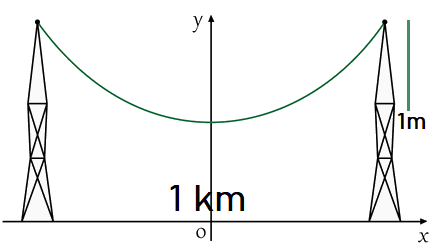
\includegraphics[width=0.3\textwidth]{catenary}
%    \end{figure*}
%
%    Solution is given by the equation
%    \[
%        \lambda \cdot \cosh\Bigl(\frac{500}{\lambda}\Bigr) - \lambda - 1 = 0
%    \]
%    Solve for $\lambda$, which can be used to compute the length of the cable
%    ($\lambda$ here is the radius of curvature at apex).
%    So, we want to find the root of this equation.
%    This is difficult to solve analytically, so we can find 
%    an approximation of $\lambda$.
%\end{example}

%\subsection{Bisection method}
%For cases like
%\begin{align*}
%    f(x) &= 12 x^2 - 5x - 2 = 0\\
%    &=(4x + 1)(3x - 2q)
%\end{align*}
%we can solve using the formula, and get $x_1 = -\frac{1}{4},\ x_2 = \frac{2}{3}$.
%But this does not work for a more complex problem, e.g.
%$f(x) = \log(3 + x^4) + 3\sin(x) = 0$.

%\begin{itemize}
%    \item {
%        We need to find an algorithm that gives a \textit{robust}
%        root localization (has to work for any nonlinear function).
%    }
%    \item {
%        We don't know how many roots there are. The algorithm should find at least one root per search.
%    }
%\end{itemize}


\pagebreak
\section{Nonlinear equations}
Linear equations can be represented by a matrix. On the other hand, nonlinear equations can't.
Nonlinear equations are about finding roots. They appear in many applications.

\begin{example}
    If we want to solve
    \[ x^2 + 3x + 7 = \log(x) \]
    If we bring it all to one side, then we have to find the root of a function.
    \[ x^2 + 3x + 7 - \log(x) = 0 \]
    Unfortunately, non-linear equations are difficult to solve analytically.
    We can usually approximate the solution by using iterative methods.
\end{example}

\subsection{Bisection method}
\begin{theorem}
    Let $f \in \operatorname{C}([a, b])$ ($f(x)$ is continuous on $[a, b]$)
    with $f(a) \cdot f(b) < 0$ (i.e. $f$ has different signs on its ends).
    Then, by continuity, there exists $r \in (a, b)$, such that
    $f(r) = 0$.
\end{theorem}
\begin{remark}
    Actually, this theorem tells that any point between $f(a)$ and $f(b)$ will be achieved.
\end{remark}

\textbf{Idea of the bisection method:}
\begin{enumerate}
    \item {
        Bisection of $[a, b]$ into $[a, c] \cup [c, b]$, i.e.
        into two subintervals, $a < c < b$.
    }
    \item {
        If $f(c) = 0$, then $r = c$, we have found the solution.
    }
    \item {
        If $f(c) \cdot f(a) < 0$, then continue with $[a, c]$.
    }
    \item {
        If $f(c) \cdot f(b) < 0$, continue with $[c, b]$.
    }
\end{enumerate}
\begin{remark}
    When $f(a) \cdot f(b) > 0$, $f$ may or may not have a root on $[a, b]$ ---
    we cannot say for sure.
\end{remark}
\begin{remark}
    This algorithm will only find one root, not all.
\end{remark}

\textbf{The method in short:}

Producing a sequence of intervals $[a_i, b_i]$ such that a root $r$ is inside these intervals.
The starting interval is $[a, b] = [a_0, b_0]$.

\begin{theorem}
    The bisection method, when applied to $[a, b]$ and 
    $f \in C^*([a, b])$ with $f(a) \cdot f(b) < 0$ will complete after
    $n$ steps an approximation $c_n$ of root $r$ with error
    \[ \abs{r - c_n} < \frac{b - a}{2^n} \]
\end{theorem}
\begin{remark}
    If we do infinitely many iterations, we will always find the root, because
    \[ \lim_{n \to \infty} \frac{b - a}{2^n} = 0 \]
\end{remark}
\begin{proof}
    At every step, the length of the interval where the root is located
    is divided into two. We can use induction to prove the above-mentioned error formula.
\end{proof}

\begin{example}
    Let $[a, b] = [0, 1]$. How many iterations are needed to decrease the error
    below $2^{-20} \approx 10^{-6}$?

    We need to find an $n \in \mathbb{N}$, such that our error estimate
    is less than what we want:
    \begin{align*}
        &
        \frac{b - a}{2^n} < 2^{-20} \Longleftrightarrow
        \frac{b - a}{2^{-20}} < 2^n \Longleftrightarrow
        \log_2\Bigl(\frac{b - a}{2^{-20}}\Bigr) 
        \overset{\text{$\log_2$ is strictly increasing}}{<} \log(2^n) = n
        \\&
        \log_2\Bigl(\frac{1}{2^{-20}}\Bigr) < n \Longleftrightarrow
        \log_{2}(1) - \log_{2}(2^{-20}) < n \Longleftrightarrow
        0 - (-20) < n \Longleftrightarrow 20 < n
    \end{align*}
\end{example}
\begin{remark}
    The bisection method has a slow convergence.
    For every iteration step we get a \textit{binary} digit as our accuracy increase.
    Recall that for approximating $\cos(x)$ by Taylor polynomial,
    we get 2 decimal digits per term of the polynomial. 
\end{remark}

\subsection{Newton method}

\begin{definition}
    Suppose that the sequence $\{x_n\}$ converges as $n \to \infty$.
    Then the sequence:
    \begin{enumerate}[label=\alph*)]
        \item {
            converges \textit{linearly} to $r$, if 
            there exists such an $M \in (0, 1)$, such that
            \[ \lim_{n \to \infty} \frac{\abs{x_{n + 1} - r}}{\abs{x_{n} - r}} = M \]
            \begin{example}
                For bisection method $M = \frac{1}{2}$.
            \end{example}
        }
        \item {
            converges \textit{super-linearly} to $r$, if
            \[ \lim_{n \to \infty} \frac{\abs{x_{n + 1} - r}}{\abs{x_{n} - r}} = 0 \]
        }
        \item {
            converges \textit{sub-linearly} to $r$, if
            \[ \lim_{n \to \infty} \frac{\abs{x_{n + 1} - r}}{\abs{x_{n} - r}} = 1 \]
            (i.e. at some point the error decrease rate stagnates).
        }
        \item {
            converges \textit{with order $q > 1$}, if there exists $M > 0$, such that
            \[ \lim_{n \to \infty} \frac{\abs{x_{n + 1} - r}}{\abs{x_{n} - r}^q} < M \]
            If $q = 2$, the convergence is called \textit{quadratic},
            if $q = 3$ --- cubic.
        }
    \end{enumerate}
\end{definition}

\begin{definition}[Newton method]
    Let $f \in \operatorname{C}^1([a, b])$. Then at every 
    $x_0 \in (a, b)$ there exists a tangent to the graph of $f$.
    The tangent equation at $x_0$ can be written as follows:
    \begin{align*}
        &
        t(x) = f(x_0) + f'(x_0)(x - x_0)
        \\&
        \frac{t(x) - f(x_0)}{x - x_0} = f'(x_0)
    \end{align*}
    If we recall, the tangent at $x_0$ is the first order Taylor polynomial of $f(x)$
    with $t(x_0) = f(x_0),\ t'(x) = f'(x_0)$.
    \pagebreak
    \begin{figure*}[h]
        \centering
        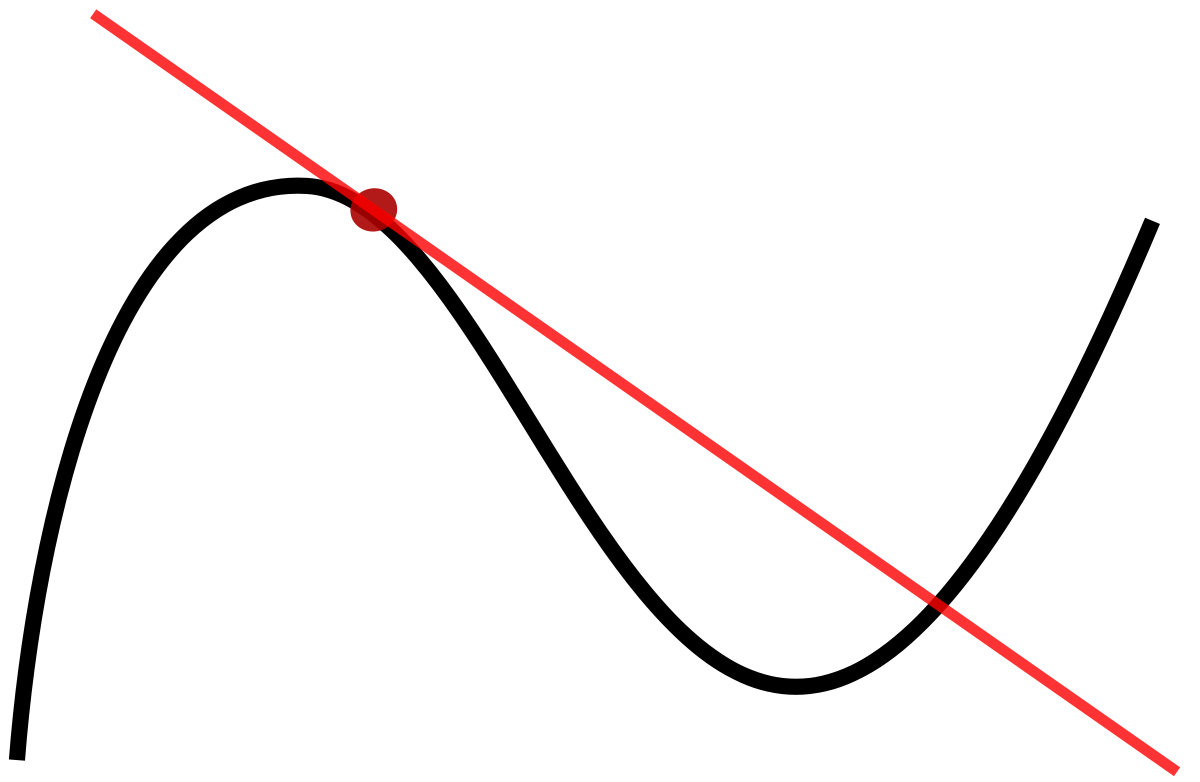
\includegraphics[width=0.3\textwidth]{tangent}
    \end{figure*}

    We use the tangent $t(x)$ as an approximation to $f(x)$,
    and we can find the root of $t(x)$ easily, as it's a linear funciton:
    \[
        0 = t(x_1) = f(x_0) + f'(x_0)(x_1 - x_0) \Longleftrightarrow
        x_1 = x_0 - \frac{f(x_0)}{f'(x_0)}
    \]

    Continuing yields the Newton sequence (Newton–Raphson iteration):
    \[ x_{n + 1} = x_n - \frac{f(x_n)}{f'(x_n)},\ x_0 = \text{initial guess} \]

    \begin{figure*}[h]
        \centering
        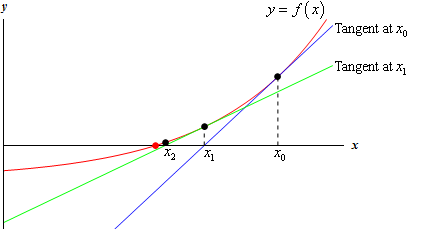
\includegraphics[width=0.5\textwidth]{newton}
    \end{figure*}

    Here we cannot have $f'(x_n) = 0$, since we cannot divide by zero. Therefore,
    it's often a good idea to make sure $f'$ doesn't have roots on the interval
    of search.
\end{definition}
\begin{theorem}
    When the Newton sequence converges, it converges to
    \textbf{a} root of $f$.
\end{theorem}
\begin{theorem}
    Suppose we have a function $f \in \operatorname{C}^2([a, b])$, such that:
    \begin{enumerate}
        \item {
            $f(a) \cdot f(b) < 0$ (there's a sign switch).
        }
        \item {
            $f$ has no critical points in $(a, b)$ (i.e. $f'(x) \ne 0$ for $x \in (a, b)$).
        }
        \item {
            $f''$ exists, is continuous and either $f'' > 0$
            or $f'' < 0$ on the whole $(a, b)$.
            I.e., $f$ is either concave down or concave up.
        }
    \end{enumerate}
    Then $f(x) = 0$ has \textit{exactly one} solution $r$. 
    The Newton sequence always converges to $r$.

    For $n \to \infty$, when the initial guess should be chosen according to:
    \begin{itemize}
        \item {
            If $f(a) < 0$, $f'' < 0$ or $f(a) > 0, f'' > 0$
            then $x_0 \in [a, r]$, e.g. $x_0 = a$.
        }
        \item {
            If $f(a) < 0$, $f'' > 0$ or $f(a) > 0$, $f'' < 0$ then
            $x_0 \in [r, b]$, e.g. $x_0 = b$.
        }
    \end{itemize}
    (If we chose an initial guess on the wrong side of the graph, then 
    the Newton method may diverge outside the domain area of  $(a, b)$ --- we don't want that.)

    In any case we have the estimate
    \[ \abs{x_n - r} < \frac{f(x_n)}{\min_{[a, b]} \abs{f'(x)}} \]
\end{theorem}

Problems with the Newton method:
\begin{enumerate}
    \item {
        The runaway problem: the Newton method may start stepping in the wrong side.
        \begin{figure*}[h]
            \centering
            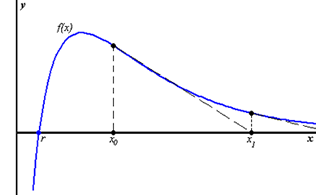
\includegraphics[width=0.5\textwidth]{runaway}
        \end{figure*}
    }
    \item {
        If we have a flat point, we don't know in which direction to go:
        \begin{figure*}[h]
            \centering
            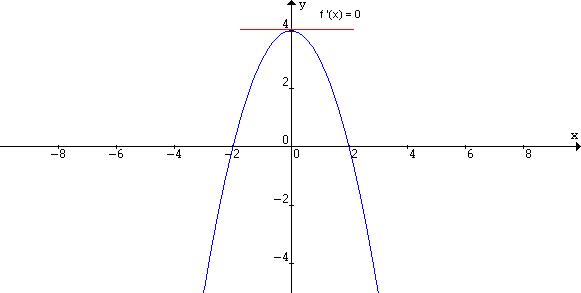
\includegraphics[width=0.5\textwidth]{flat_point}
        \end{figure*}
    }
    \item {
        Sometimes the Newton method can jump infinitely between two points in a cycle
        without ever converging.
        \begin{figure*}[h]
            \centering
            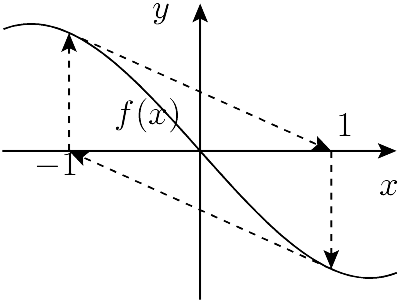
\includegraphics[width=0.5\textwidth]{newton_cycle}
        \end{figure*}
    }
\end{enumerate}
\pagebreak
\begin{theorem}
    If $f : [a, b] \to \mathbb{R}$ fullfills:
    \begin{enumerate}
        \item {
            $f(a) \cdot f(b) < 0$.
        }
        \item {
            $f$ has no critical points in $(a, b)$.
        }
        \item {
            $f''$ exists and is continuous ($f \in \operatorname{C}^2([a, b])$)
            and $x_0$ is \textit{``close enough''} (not a mathematical term)
            to the root $r$.
        }
    \end{enumerate}
    Then the Newton sequence converges quadratically.
\end{theorem}
\begin{proof}
    We have to show that
    $\abs{x_{n + 1} - r} \le M \abs{x_n - r}^2$ as $n \to \infty$.
    By Taylor series approximation,
    \[ 
        f(x) = f(x_n) + f'(x_n)(x - x_n) + \frac{1}{2} f''(\xi_n)(x - x_n)^2 
        \text{, where } \xi_n \in (x, x_n)
    \]
    Since $r$ is a root of $f$, when we put $x = r$, we get
    \[
        0 = f(r) = f(x_n) + f'(x_n)(r - x_n) + \frac{1}{2} f''(\xi_n)(r - x_n)^2
    \]
    Let's divide both sides by $f'(x_n)$ and rearrange the terms:
    \begin{align*}
        &\frac{f(x_n)}{f'(x_n)} +
        \frac{f'(x_n)}{f'(x_n)} (r - x_n) = -\frac{f''(\xi_n)}{2 f'(x_n)}(r-x_n)^2
        \\&\Longleftrightarrow (r - x_{n+1}) = -\frac{f''(\xi_n)}{2 f'(x_n)} (r - x_n)^2
        \quad \Bigl(x_{n+1} = x_n - \frac{f(x_n)}{f'(x_n)}\Bigr)
        \\&\implies \abs{r - x_{n+1}} = \abs{\frac{f''(\xi_n)}{2f'(x_n)}} \abs{r - x_n}^2
    \end{align*}
    Let
    \[ M \coloneqq \sup_{x_n,\, \xi_n} \abs{\frac{f''(\xi_n)}{2f'(x_n)}} \]
    The supremum will be finite, because $x_n$ and $\xi_n$ are both
    inside bounded intervals.

    Then $\abs{r - x_{n + 1}} \le M \abs{r - x_n}^2$.
\end{proof}
\begin{remark}
    We need $x_0$ to be close enough to make sure the Newton method
    doesn't go outside the domain $[a, b]$.
\end{remark}

\subsection{Modifications of the Newton method}
\subsubsection{Modified Newton method}
As we remember, in the usual Newton method
\[ x_{n+1} = x_n - \frac{f(x_n)}{f'(x_n)} \]
If $f'(x_n)$ doesn't change much anymore from $n$ to $n + 1$, we can fix it to
$f'(x_m)$ with some fixed $m \le n$. Then our new formula for $x_{n+1}$ is
\[ x_{n + 1} = x_n - \frac{f(x_n)}{f'(x_m)} \]
We avoid futher evaluations of $f'(x)$ which saves computational resources.

\subsubsection{Secant method}
Newton's method needs derivatives. 
We can approximate the derivatives by secants (also called a difference quotient):

\[
    f'(x) = \lim_{h \to 0} \frac{f(x + h) - f(x)}{h} \implies
    f'(x) \approx \frac{f(x + h) - f(x)}{h} \text{ for small $h$}
\]
For the Secant method, we let $x_n \coloneqq x_n,\ h \coloneqq x_{n - 1} - x_{n}$.
\[ f'(x_n) \approx \frac{f(x_{n - 1}) - f(x_n)}{x_{n - 1} - x_{n}} \]
Substitution into Newton method gives us
\[ x_{n + 1} = x_{n} - \frac{f(x_n) (x_{n - 1} - x_{n})}{f(x_{n - 1}) - f(x)} \]

The Secant method converges slower than the Newton method, but it's easier to compute.

\begin{theorem}
    If $f \in \operatorname{C}^2([a, b])$
    and $r \in (a, b),\ f(r) = 0,\ f'(r) \ne 0$
    and 
    \[ x_{n + 1} = x_n - \frac{f(x_n) (x_{n-1} - x_n)}{f(x_{n - 1} - f(x_n))} \]
    Then there exists a $\delta > 0$, such that for every $x_1, x_0$, such that
    $\abs{r - x_1} < \delta$, $\abs{r - x_0} < \delta$, we'll have
    \begin{enumerate}
        \item {
            $\lim_{n \to \infty} \abs{x_n - r} = 0$ (the sequence converges)
        }
        \item {
            $\abs{r - x_{n + 1}} \le M \abs{r - x_n}^\alpha$
            with $\alpha = \frac{1 + \sqrt{5}}{2} \approx 1.618$
            (the sequence converges with order of golden ratio).
        }
    \end{enumerate}
\end{theorem}
\begin{example}
    \[ f(x) = x^5 - 3x + 1 = 0,\ f'(x) = 5x^4 + 3 \]
    Newton method:
    \begin{align*}
        &x_0 = 0,\ f(0) = 1,\ f'(0) = 3
        \\&
        x_1 = x_0 = \frac{f(x_0)}{f'(x_0)} = 0 - \frac{1}{3} = -\frac{1}{3}
    \end{align*}

    Secant method:
    \begin{align*}
        &x_0 = 1,\ x_1 = \frac{1}{2}
        \\&
        x_2 = \frac{1}{2} - \frac{f(1/2)(1 - 1/2)}{f(1) - f(1/2)} = \dots
    \end{align*}
\end{example}

Summary:
{
\scriptsize
\[\begin{array}{c|c|c|c|c|c}
    & \text{\#initials} & \text{Regularity of $f$} & \text{Convergence} & \text{Root between points} & \text{Function calls per iteration}
    \\\hline
    \text{Bisection} & \text{2 ($a$, $b$)} & \operatorname{C}([a, b]) & \text{linear} & \text{Yes} & 1
    \\\hline
    \text{Newton} & \text{1 ($x_0$)} & \operatorname{C^2}([a, b]) &
    \text{quadratic} & \text{No} & 2
    \\\hline
    \text{Secant} & \text{2 ($x_0$, $x_1$)} & \operatorname{C^2}([a, b]) &
    \text{superlinear/order $\alpha = 1.618$} & \text{No} & 1
\end{array}
\]
}
\begin{theorem}[Simple approximation theorem]
    $f: E \to \overline{\mathbb{R}}$ is measurable if and only if 
    there exists a sequence of simple functions $\varphi_n : E \to \mathbb{R}$,
    such that $\varphi_n \to f$ pointwise on $E$, and $\abs{\varphi_n} \le \abs{f}$
    on $E$ for all $n$.

    (If $f \ge 0$, then $\{\varphi_n\}$ can be chosen to be increasing.)
\end{theorem}
\begin{remark}
    In the simple approximation lemma, functions 
    $\varphi_\varepsilon$ and $\psi_\varepsilon$ sandwich the function $f$,
    and\\ $0 \le \psi_\varepsilon - \varphi_\varepsilon < \varepsilon$, therefore, 
    at every point they both differ from $f$ by no more than $\varepsilon$.
    If we could choose a sequence of $\varepsilon$'s that converges to 0,
    we would get uniform convergence.

    Unfortunately, we can't apply the lemma directly, because we needed the function $f$ to be bounded.
    That's why we're not getting uniform convergence.
\end{remark}
\begin{proof}
    \begin{enumerate}
        \item {
            $\impliedby$. We have a sequence of simple (and thus measurable) functions $\{\varphi_n\}$,
            therefore, their limit is also measurable.
        }
        \item {
            $\implies$.
            \begin{enumerate}[label={(\arabic*)}]
                \item {
                    Let's express $f = f^+ - f^-$, where $f^+ = \max\{f, 0\}$ and $f^- = \min\{f, 0\}$.
                    Let's prove the theorem for both $f^+$ and $f^-$.
                    Without the loss of generality, assume that $f \ge 0$.
                }
                \item {
                    To use the simple approximation lemma, we have to make the function bounded.
                    Define $f_n \coloneqq \min\{f, 2^n\}$.
                    Take $\varphi_n$ as the lower simple approximation of $f_n$,
                    according to the simple approximation lemma, with $\varepsilon = \frac{1}{2^n}$.

                    Then $\varphi_n \to f$ pointwise. Moreover, $\{\varphi_n\}$ 
                    are increasing (because we bound it with $2^n$, and because when we 
                    go from $n$ to $n + 1$, every interval in the proof of SAL is split into two).
                }
                \item {
                    Do the same for $f^-$ and add the sequences for $f^+$ and $f^-$ together.
                    Since $\abs{f} = \max\{\abs{f^+}, \abs{f^-}\}$, the condition
                    of $\abs{\varphi_n} \le \abs{f}$ will hold true. 
                }
            \end{enumerate}
        }
    \end{enumerate}
\end{proof}

\subsection{Egoroff, Lusin, Littlewood's three principles}
Informal statement:
\begin{enumerate}
    \item {
        Every measurable set is \textit{nearly} (not a mathematical term) a finite union of intervals.
    }
    \item {
        Every measurable function is nearly continuous.
    }
    \item {
        Every pointwise convergent sequence of measurable functions is nearly uniform convergent.
    }
\end{enumerate}
\begin{theorem}[Egoroff's theorem]
    Assume that $m(E) < \infty$, 
    $f_n : E \to \overline{\mathbb{R}}$ --- measurable, $f_n \to f$
    pointwise almost everywhere on $E$, where $f : E \to \mathbb{R}$.
    Then for any $\varepsilon > 0$ there exists a closed subset
    $F \subset E$, such $m(E \setminus F) < \varepsilon$ and $f_n \to f$
    uniformly on $f$.
\end{theorem}
\begin{remark}
    It is crucial that $f$ is from $E$ to $\mathbb{R}$, not $\mathbb{\overline{R}}$,
    otherwise we wouldn't get uniform convergence.
\end{remark}
\begin{proof}
    $\abs{f} < \infty \implies \abs{f - f_k}$ is defined for all $x \in E$
    (starting from some $k$).

    Let's also throw out the subset of measure $E$, on which $f_n \not\to f$.

    \begin{enumerate}
        \item {
            Fix $\eta > 0$.
            \[ E_n \coloneqq \{ x \in E \mid \abs{f(x) - f_k(x)} < \eta,\ \forall k \ge n \} \]
            Each set $E_n$ is measurable, because $\abs{f(x) - f_k(x)}$ is measurable,
            and $E_n$ is the countable intersection of preimages of $[0, \eta)$ for all $k$.
            We can also note that $\{E_n\}$ is ascending.
            
            Also, $ \cup_{n=1}^\infty E_n = E $.
            That's follows from pointwise convergence. If we take any point from the set $E$,
            eventually it will be contained in some $E_n$, because for a given point $x$
            the difference $\abs{f(x) - f_k(x)}$ has to converge to 0. 
            Therefore,
            \[
                \lim_{n \to \infty} m(E_n) = m(E)
            \]
            Then there exists $N \in \mathbb{N}$, such that 
            $m(E \setminus E_n) < \varepsilon$ for every $\varepsilon > 0$.
        }
        \item {
            Now let's take such $N$ for $\eta_n = \frac{1}{n}$,
            $\varepsilon_n = \frac{\varepsilon}{2^{n + 1}}$.

            Take $E_n = E_N$, where $E_N$ is from step 1
            for $\eta = \eta_n$ and $\varepsilon = \varepsilon_n$.

            Take $A = \cap_{n=1}^\infty E_n$. Then
            $f_n \to f$ uniformly on $A$. On the other hand, 
            $A$ is measurable as a countable union of measurable sets.

            Let's estimate the measure of $A$.
            \[ m(E \setminus A) = m\Bigl(
                \bigcup_{k=1}^\infty (E \setminus E_n)
            \Bigr) \le
            \sum_{n=1}^\infty m(E \setminus E_n) \le
            \sum_{n=1}^\infty \frac{\varepsilon}{2^{n+1}} = \frac{\varepsilon}{2}
            \]
            But $A$ may be non-closed, so we can't just assign $F$ to $A$.
            Therefore, we have to approximate $A$ by closed sets.
        }
        \item {
            Take $F \subset A$, so that $F$ is closed and
            $m(A \subset F) < \frac{\varepsilon}{2}$.
            We \hyperref[the:lebesgueMeasurableConditions]{have proved} that such an $F$ exists if $A$ is measurable.
        }
    \end{enumerate}
\end{proof}

\begin{theorem}[Lusin's theorem]
    $f : E \to \mathbb{R}$ --- measurable. Then for every
    $\varepsilon > 0$ there exists a continuous function
    $g : \mathbb{R} \to \mathbb{R}$ and a closed set $F \subset E$, 
    such that $f = g$ on $F$ and $m(E \setminus F) < \varepsilon$.
\end{theorem}
\begin{proof}
    \textit{Main idea}: uniform limit of continuous functions is continuous,
    then apply Egoroff's theorem.

    The proof is gonna be split into two parts:
    \begin{enumerate}
        \item {
            Find a closed $F$ on which $f$ is continuous (in induced topology).
        }
        \item {
            Extend $f|_F$ to a continuous function $g$.
            We have briefly discussed how to do this:
            the complement of a closed set $F$ is an open set, 
            and thus a disjoint union of open intervals. On every such
            open interval we can connect the graph of $f$
            with a straight line. There's some work to be done, because
            there can be an infinite number of such intervals converging a point,
            but we'll leave it as an exercise.
        }
    \end{enumerate}

    Proof of Part 1:
    \begin{enumerate}
        \item {
            Assume $m(E) < \infty$. (Let's leave $m(E) = \infty$
            as an exercise).
            By simple approximation lemma, there exists a sequence of 
            simple functions $f_n : E \to \mathbb{R}$, such that
            $f_n \to f$ pointwise.
        }
        \item {
            $\forall n$ there exists a closed subset $F_n \subset F$,
            such that $f_n$ is continuous on $F_n$ and
            $m(E \setminus F_n) < \frac{\varepsilon}{2^{n+1}}$.
            
            Proof:
            \[ f_n = \sum_{j=1}^{k_n} c_j \cdot \chi_{E_j} \text{ --- canonical representation} \]
            Each of the sets $E_j$ 
            \hyperref[the:lebesgueMeasurableConditions]{can be approximated}
            by a closed set $G_j$ from the inside (they are measurable from
            \hyperref[def:simpleFunction]{the definition of a simple function}).

            Put $F_n \coloneqq \cup G_j$. It's a finite union, therefore $F_n$ is closed.

            $f_n$ is constant on each of $G_j$, as $G_j \subset E_j$.
            A preimage of an open set for $f$ was a union of several $E_j$'s.
            If we now restrict $f$ onto $\cup G_j$, the preimage of an open set
            will be a union of several $G_j$'s. What we have to prove that 
            $G_j$'s are open in the induced topogy on $F_n$ --- that's 
            true because $G_j$'s are closed in $\mathbb{R}$ and disjoint.
        }
        \item {
            By Egoroff's theorem, there exists a closed $F_0 \subset E$, 
            such that $m(E \setminus F_0) < \frac{\varepsilon}{2}$ and 
            $f_n \to f$ uniformly.
            Now take $F \coloneqq \cap_{n=0}^\infty F_n$. The intersection of closed sets 
            is closed. 
            By construction, $f_n$ is continuous on $F$, as $F_n \subset F$.
            Since $f_n \to f$ uniformly on $F$ (as $F_0 \subset F$),
            $f$ is continuous on $F$.
            Let's now estimate the measure of $E \setminus F$:
            \[
                m(E \setminus F) < \frac{\varepsilon}{2} + 
                \sum_{n=1}^\infty \frac{\varepsilon}{2^{n+1}} = \varepsilon
            \]
        }
    \end{enumerate}
\end{proof}
\begin{remark}
    If $m(E) = \infty$, we can split $\mathbb{R}$ into intervals with finite length.
    Then use the finite case we've just proved for each of those intervals,
    but choose $\varepsilon_k = \frac{\varepsilon}{2^{k + 1}}$ so that they all sum 
    up to $\varepsilon$ at the end.
\end{remark}

\pagebreak
\section{Lebesgue integral}
\begin{definition}
    Let $\psi : E \to \mathbb{R}$ be simple, $m(E) < \infty$. Let
    \[ \psi = \sum_{n=1}^k a_n \cdot \chi_{E_n} \]
    be the canonical representation of $\psi$. Then define
    \[ \int_E \psi \coloneqq \sum_{n=1}^k a_n \cdot m(E_n) \]
\end{definition}
\begin{remark}
    Notation: if we want to emphasize the measure, we can write
    \[ \int_E \psi = \int_E \psi \,dm = \int_a^b \psi \,dm \text{ (when $E=[a, b]$)} \]
\end{remark}
\begin{remark}
    One can show that if it's not the canonical representation,
    we can still compute the integral by the same formula and get the same result.
\end{remark}

\begin{definition}
    Let $f : E \to \mathbb{R}$ be bounded, $m(E) < \infty$.
    ($f$ is not necessarily measurable).

    The \textit{lower Lebesgue integral} is by definition
    \[ \sup\Bigl\{ \int_E \varphi \mathrel{\Big\vert} \text{ $\varphi$ is simple and $\varphi \le f$ on $E$} \Bigr\} \]
    The \textit{upper Lebesgue integral} is by definition
    \[ \inf\Bigl\{ \int_E \psi \mathrel{\Big\vert} \text{ $\varphi$ is simple and $\varphi \ge f$ on $E$} \Bigr\} \]
    $f$ is \textit{Lebesgue integrable} if the lower Lebesgue integral
    is equal to the upper Lebesgue integral. Then
    \[ \int_E f \coloneqq \text{lower Lebesgue integral} = \text{upper Lebesgue integral} \]
\end{definition}

\begin{theorem}
    $f : [a, b] \to \mathbb{R}$ is bounded and $[a, b]$ is bounded.
    If $f$ is Riemann integrable over $[a, b]$, then 
    $f$ is Lebesgue integrable and both integrals will match.
\end{theorem}
\begin{proof}
    Upper and lower Riemann sums are obtained by simple functions.
\end{proof}
\begin{theorem}
    If $f : E \to \mathbb{R}$ is bounded and \textit{measurable}, 
    $m(E) < \infty$, then $f$ is Lebesgue integrable on $E$.
\end{theorem}
\begin{proof}
    By the simple approximation lemma, for every $n \in \mathbb{N}$
    there exist simple functions $\varphi_n$, $\phi_n$, such that
    $\varphi_n \le f \le \psi_n$ on $E$ and
    $\psi_n - \varphi_n \le \frac{1}{n}$ on $E$.
    \[
        \forall n: 
        (\text{upper Lebesgue integral} - \text{lower Lebesgue integral}) \le
        \int_E \psi_n - \int_E \varphi_n = \int_E (\psi_n - \varphi_n) \le
        \frac{1}{n} m(E) \to 0
    \]
    Here we've used the fact that the difference of two integrals
    is the integral of the difference (which we haven't yet proved).
    However, since we're dealing with simple functions,
    we can prove it by simply rearranging the finite sums.
\end{proof}

Now here's some definitions for the improper case,
i.e. infinite integration limits or functions that converge to infinity.

\begin{definition*}
    $f : E \to \overline{\mathbb{R}}$ is measurable.
    Its support is by definition
    \[ \supp f \coloneqq \{ x \in E \mid f(x) \ne 0 \} \]
    $f$ is of finite support of $m(\supp f) < \infty$.
\end{definition*}
\begin{definition}
    \label{def:definitionThree}
    $f : E \to \overline{\mathbb{R}}$ is measurable, $f \ge 0$. Then
    \[
        \int_E f \coloneqq \sup \Bigl\{
            \int_E h \mathrel{\Big\vert}
            \text{$h$ is bounded, measurable,}\
            m(\supp h) < \infty,\ 0 \le h \le f \text{ on } E
        \Bigr\} 
    \]
    $f$ is Lebesgue integrable over $E$, if $\int_E f < \infty$.
\end{definition}
\begin{definition}
    A measurable function $f : E \to \overline{\mathbb{R}}$
    is Lebesgue measurable over $E$ if 
    $f^+ = \max\{f, 0\}$ and $f^- = \max\{-f, 0\}$ are Lebesgue
    integrable over $E$.
    Then
    \[ \int_E f = \int_E f^+ - \int_E f^- \]
\end{definition}

\end{document}
